\documentclass[12pt, a4paper]{report}

% ── Packages ──────────────────────────────────────────────
\usepackage[a4paper, margin=2.5cm]{geometry}
\usepackage{graphicx}
\usepackage{booktabs}
\usepackage{array}
\usepackage{amsmath}
\usepackage{amssymb}
\usepackage{hyperref}
\usepackage{setspace}
\usepackage{titlesec}
\usepackage{fancyhdr}
\usepackage{xcolor}
\usepackage{enumitem}
\usepackage{caption}
\usepackage{float}
\usepackage{parskip}
\usepackage{tocloft}
\usepackage{listings}
\usepackage{mdframed}

% ── Colors ────────────────────────────────────────────────
\definecolor{iiitblue}{RGB}{0, 56, 101}
\definecolor{teal}{RGB}{2, 128, 144}
\definecolor{lightgray}{RGB}{245, 245, 245}
\definecolor{darkgray}{RGB}{80, 80, 80}

% ── Hyperref setup ────────────────────────────────────────
\hypersetup{
    colorlinks=true,
    linkcolor=iiitblue,
    citecolor=teal,
    urlcolor=teal,
    pdftitle={Improving SDN Forensic Data Storage using Cuckoo Filters},
    pdfauthor={Kuldeep Kumar Lakhe, Atharva Keskar, Dheeraj Makhija}
}

% ── Font & Spacing ────────────────────────────────────────
\onehalfspacing

% ── Section title formatting ──────────────────────────────
\titleformat{\chapter}[display]
  {\normalfont\Large\bfseries\color{iiitblue}}
  {\chaptertitlename\ \thechapter}{12pt}{\Huge}
\titlespacing*{\chapter}{0pt}{0pt}{20pt}

\titleformat{\section}
  {\normalfont\large\bfseries\color{iiitblue}}
  {\thesection}{1em}{}

\titleformat{\subsection}
  {\normalfont\normalsize\bfseries\color{darkgray}}
  {\thesubsection}{1em}{}

% ── Header / Footer ───────────────────────────────────────
\pagestyle{fancy}
\fancyhf{}
\fancyhead[L]{\small\textcolor{darkgray}{SDN Forensic Data Storage using Cuckoo Filters}}
\fancyhead[R]{\small\textcolor{darkgray}{IIIT Hyderabad}}
\fancyfoot[C]{\thepage}
\renewcommand{\headrulewidth}{0.4pt}

% ── Table of Contents dots ────────────────────────────────
\renewcommand{\cftchapdotsep}{\cftdotsep}

% ── Code listing style ────────────────────────────────────
\lstset{
  basicstyle=\ttfamily\small,
  backgroundcolor=\color{lightgray},
  frame=single,
  breaklines=true,
  keywordstyle=\color{iiitblue}\bfseries,
  commentstyle=\color{darkgray},
  numbers=left,
  numberstyle=\tiny\color{darkgray},
  xleftmargin=2em
}

% ── Info box ──────────────────────────────────────────────
\newmdenv[
  backgroundcolor=lightgray,
  linecolor=teal,
  linewidth=2pt,
  leftline=true,
  rightline=false,
  topline=false,
  bottomline=false,
  innerleftmargin=12pt,
  innerrightmargin=8pt,
  innertopmargin=8pt,
  innerbottommargin=8pt
]{infobox}

% ══════════════════════════════════════════════════════════
\begin{document}

% ── TITLE PAGE ────────────────────────────────────────────
\begin{titlepage}
\centering

\vspace*{0.5cm}

% Institute name
{\Large\bfseries\color{iiitblue}
International Institute of Information Technology\\[4pt]
Hyderabad, India
\par}

\vspace{0.5cm}
\textcolor{teal}{\rule{\linewidth}{2pt}}
\vspace{0.5cm}

% Title
{\Huge\bfseries\color{iiitblue}
Improving SDN Forensic\\[8pt]
Data Storage using\\[8pt]
Cuckoo Filters
\par}

\vspace{0.6cm}
\textcolor{teal}{\rule{\linewidth}{1pt}}
\vspace{-0.6cm}

% Subject
{\large\textit{PG Project Report}\\[2pt]


\vspace{1cm}

% Authors box
\begin{mdframed}[linecolor=teal, linewidth=1.5pt, roundcorner=6pt,
  innertopmargin=14pt, innerbottommargin=14pt]
\centering
{\large\bfseries Submitted by}\\[10pt]
\begin{tabular}{ll}
\textbf{Kuldeep Kumar Lakhe} & Roll No: 2024202025 \\[4pt]
\textbf{Atharva Keskar}      & Roll No: 2024202017 \\[4pt]
\textbf{Dheeraj Makhija}     & Roll No: 2024202011 \\
\end{tabular}
\end{mdframed}

\vspace{0.8cm}

% Guide box
\begin{mdframed}[linecolor=iiitblue, linewidth=1.5pt, roundcorner=6pt,
  innertopmargin=12pt, innerbottommargin=12pt]
\centering
{\large\bfseries Under the Guidance of}\\[8pt]
{\large\textbf{Prof.\ Shatrunjay Rawat}}\\[4pt]
{\normalsize International Institute of Information Technology, Hyderabad}\\
{\normalsize \texttt{shatrunjay.rawat@iiit.ac.in}}
\end{mdframed}

\vfill

{\normalsize\textcolor{darkgray}{April 2026}}

\end{titlepage}



% ── ABSTRACT ──────────────────────────────────────────────
\newpage
\thispagestyle{plain}
\chapter*{Abstract}
\addcontentsline{toc}{chapter}{Abstract}

Network forensic analysis in Software Defined Networking (SDN) environments
depends critically on the continuous availability of forensic log data.
Existing approaches, notably the work by Sharma and Rawat, use Bloom Filters
to store and compress SDN forensic logs efficiently. However, Bloom Filters
suffer from a fundamental limitation: they do not support selective deletion
of individual entries. When a Bloom Filter reaches capacity, the entire filter
must be wiped and reset, resulting in complete and irreversible loss of all
stored forensic evidence. Furthermore, even Cuckoo Filter-based approaches
that use sliding window deletion are forensically unsound, as modifying
forensic logs violates evidence immutability requirements.

This project proposes a three-tier improvement over existing approaches.
First, we replace Bloom Filters with Cuckoo Filters and implement an
\textit{Attack-Aware Sliding Window} retention policy. Second, we introduce
a \textbf{Forensic Filter Manager} that uses a \textit{Snapshot + Reset}
archival model: when a filter approaches capacity, it is serialized to disk
as an immutable snapshot and a fresh filter is created --- ensuring that
forensic evidence is \textbf{never deleted or modified}. Third, we extend
the SDN topology from a linear chain to a realistic \textbf{hierarchical
tree topology} (core--aggregation--access) and simulate
\textbf{multiple simultaneous attacks} from different sources.
We implement two complementary traceback mechanisms: (i)~a Source Path
Isolation-style \textbf{query-all} traceback, and (ii)~a
\textbf{parent-pointer walk-back} in which each router remembers which
upstream router handed it the packet, allowing the victim (through an SDN
controller) to reconstruct the exact ordered attack path. The entire pipeline
is evaluated on the CIC-IDS2017 benchmark dataset containing real-world
FTP-Patator brute-force attacks across 50,000 packet records.

Our experiments produce six concrete findings. First, in the offline
filter comparison, the Cuckoo Filter with sliding window achieves
\textbf{96/100} traceability vs.\ \textbf{2/100} for Bloom. Second,
the \textbf{Snapshot + Reset} model achieves \textbf{100/100}
traceability with zero deletions and zero wipes --- fully forensically
sound. Third, on a \textbf{7-switch tree topology} with two simultaneous
attack types ($H_0\!\to\!H_3$ and $H_1\!\to\!H_2$), Cuckoo-based
traceback achieves \textbf{100/100} success while Bloom achieves only
\textbf{1/100}. Fourth, a \textbf{fingerprint size sweep} (8--16~bits)
shows that increasing from 10 to 16~bits reduces the false positive rate
from 0.78\% to 0.01\% at a cost of only +60\% memory per filter.
Fifth, parent-pointer traceback issues only \textbf{O(path~length)}
queries vs.\ SPIE's \textbf{O(N~switches)}, a \textbf{42\% reduction}
in a 6-switch network and \textbf{17$\times$} reduction at 50 switches.
Sixth, a scalability sweep from \textbf{N=6 to N=50} shows accuracy
remains at \textbf{99--100\%}.

\vspace{1cm}
\noindent\textbf{Keywords:} SDN, Network Forensics, Cuckoo Filter, Bloom
Filter, Forensic Immutability, Snapshot + Reset, Tree Topology,
Parent-Pointer Traceback, SPIE, SDN Controller, Attack-Aware Eviction,
Fingerprint Sweep, Scalability, CIC-IDS2017

% ── ACKNOWLEDGEMENT ───────────────────────────────────────
\newpage
\chapter*{Acknowledgement}
\addcontentsline{toc}{chapter}{Acknowledgement}

We would like to express our sincere gratitude to \textbf{Prof.\ Shatrunjay
Rawat}, our project guide at the International Institute of Information
Technology, Hyderabad, for his invaluable guidance, continuous support, and
encouragement throughout this project. His foundational research work on
network management frameworks and Bloom Filter-based SDN forensic log
retention directly inspired and shaped our contribution. The idea of
\textit{each soft router remembering which neighbour handed it the packet},
which became the parent-pointer traceback mechanism in this work, was
suggested during our project meetings with him.

We are also grateful to the Canadian Institute for Cybersecurity at the
University of New Brunswick for making the CIC-IDS2017 dataset publicly
available for research purposes.

\vspace{1cm}
\begin{flushright}
Kuldeep Kumar Lakhe\\
Atharva Keskar\\
Dheeraj Makhija\\
\vspace{4pt}
\textit{IIIT Hyderabad, April 2026}
\end{flushright}

% ── TABLE OF CONTENTS ─────────────────────────────────────
\newpage
\tableofcontents

% ── LIST OF FIGURES ───────────────────────────────────────
\newpage
\listoffigures
\addcontentsline{toc}{chapter}{List of Figures}

% ── LIST OF TABLES ────────────────────────────────────────
\listoftables
\addcontentsline{toc}{chapter}{List of Tables}

% ══════════════════════════════════════════════════════════
\newpage
\chapter{Introduction}
% ══════════════════════════════════════════════════════════

\section{Background}

Network forensics is a critical component of cybersecurity investigation,
enabling security analysts to trace the source and path of malicious network
activity after an attack has occurred. In Software Defined Networking (SDN)
environments, the centralized control plane generates and manages large
volumes of network flow logs that serve as the primary source of forensic
evidence.

The fundamental challenge in SDN forensics is storage: network traffic
generates logs at an enormous rate, and retaining all logs indefinitely is
neither technically nor financially feasible. Network providers must purge
data beyond a certain retention period, risking the loss of critical forensic
evidence for older attacks. Beyond raw storage, forensic analysis also
requires \textit{traceability} --- the ability, once an attack is detected,
to reconstruct the path the malicious packets took through the network so
that the attacker can be located and the compromise scoped.

\section{Problem Statement}

Bloom Filters have been proposed as an effective solution to this storage
problem. Integrating forensic log data into Bloom Filters reduces storage
requirements by up to 10 times compared to raw log formats, enabling longer
forensic data retention with the same hardware resources. However, Bloom
Filters suffer from a critical and well-known limitation: they do not support
the deletion of individual items.

This creates three major problems in forensic contexts:

\begin{enumerate}[leftmargin=*, label=\textbf{\arabic*.}]

  \item \textbf{Total Evidence Loss on Saturation:}
  When a Bloom Filter reaches capacity, it must be completely wiped. All
  historical forensic evidence is permanently destroyed in a single
  operation. In our offline experiment this occurred \textbf{4 times}
  across 50,000 packets; in the network experiment it occurred
  \textbf{14 times} across 6 switches.

  \item \textbf{Compliance Violations:}
  Privacy regulations such as GDPR require selective deletion of specific
  records after a defined retention period. Bloom Filters cannot achieve
  this without destroying the entire dataset.

  \item \textbf{Forensic Blind Spots:}
  The period immediately following a wipe represents a ``blind spot'' during
  which no historical evidence is available. An attacker exploiting the
  system during this window leaves no traceable record. In an SDN network,
  even if a few switches escape a wipe, the \textit{per-router chain} is
  broken at every wiped device, destroying path reconstruction.

\end{enumerate}

\section{Proposed Solution}

This project proposes replacing Bloom Filters with Cuckoo Filters as a
direct replacement for Bloom Filters in SDN forensic log storage, and then
extending the design with four new components:

\begin{itemize}[leftmargin=*]
  \item An \textbf{Attack-Aware Sliding Window} retention policy that uses
  the Cuckoo Filter's deletion capability to selectively remove only the
  oldest \textit{benign} traffic entries when capacity is approached, while
  permanently preserving all \textit{attack-marked} evidence.
  \item A \textbf{Forensic Filter Manager (Snapshot + Reset)} that
  archives full filters to disk as immutable snapshots instead of deleting
  entries, ensuring that forensic evidence is never modified or destroyed
  --- meeting legal and compliance requirements for evidence immutability.
  \item A \textbf{Parent-Pointer Traceback} mechanism in which every soft
  router additionally records the upstream switch that handed it each
  packet. A victim, working through the SDN controller, can then
  reconstruct the exact ordered attack path by walking backward through
  these pointers --- visiting only the switches on the path, rather than
  querying every switch in the network.
  \item A \textbf{Tree Topology} (core--aggregation--access) that replaces
  the original linear chain, providing a realistic hierarchical SDN
  structure with multiple simultaneous attack paths.
\end{itemize}

\section{Project Objectives}

\begin{enumerate}[leftmargin=*, label=\textbf{\arabic*.}]
  \item Develop Python implementations of both a Standard Bloom Filter and
  an Attack-Aware Cuckoo Filter for benchmarking.
  \item Process the CIC-IDS2017 real-world network dataset to simulate
  high-volume traffic ingestion including brute force attacks.
  \item Implement the Attack-Aware Sliding Window that preserves attack
  evidence while evicting only benign traffic.
  \item Develop a \textbf{Forensic Filter Manager} using the Snapshot +
  Reset model to achieve forensically sound, immutable evidence storage
  with 100\% traceability.
  \item Extend the design to a full SDN soft-router topology with both
  \textbf{linear} and \textbf{tree} (core--aggregation--access) topologies,
  where every switch carries its own Bloom and Cuckoo filters.
  \item Simulate \textbf{multiple simultaneous attacks} from different
  sources on different paths within the tree topology.
  \item Implement and compare \textit{three} forensic traceback strategies
  on this network: (a)~Bloom~$+$~SPIE query-all, (b)~Cuckoo~$+$~SPIE
  query-all, and (c)~Cuckoo~$+$~Parent-Pointer walk-back orchestrated by
  an SDN controller.
  \item Conduct a \textbf{fingerprint size sweep} (8--16~bits) to
  quantify the cost-benefit tradeoff of achieving 100\% traceability.
  \item Quantify the scalability of each method by sweeping the number of
  switches from 6 up to 50.
\end{enumerate}

\section{Report Organization}

The rest of this report is organized as follows. Chapter~2 reviews the
related work. Chapter~3 presents the proposed system design, covering
the filter layer (Bloom, Cuckoo, and Forensic Filter Manager), the
configurable fingerprint size, the tree topology, and the SDN
soft-router traceback layer. Chapter~4 describes the experimental
methodology for all six experiments. Chapter~5 presents and analyzes
the results, including the offline comparison, network traceback,
scalability sweep, three-way enhanced comparison, tree topology with
multiple attacks, and fingerprint size cost-benefit analysis. Chapter~6
discusses the implications, presents five concrete use cases, and
acknowledges limitations. Chapter~7 concludes the report with future
work directions.

% ══════════════════════════════════════════════════════════
\chapter{Related Work}
% ══════════════════════════════════════════════════════════

\section{Network Management Framework for Forensic Traceability}

Bhondele, Rawat and Renukuntla \cite{shesha2015} proposed a network
management framework for network forensic analysis that established the
foundation of content-based traceback in network forensics. Their work
introduced the concept of \textbf{payload attribution}, where each network
device stores a compressed representation of packet content using Bloom
Filters. When a malicious packet is detected, the system queries each
device's Bloom Filter using a packet ``excerpt'' to reconstruct the path
traversed by the attack.

Their framework proposed two management approaches:

\begin{itemize}[leftmargin=*]
  \item \textbf{Distributed Management Method:} Each device stores and
  queries its own Bloom Filter independently.
  \item \textbf{Centralized Management Method:} All Bloom Filters are
  aggregated at a central Network Management System (NMS) for processing.
\end{itemize}

This work is foundational to our project as it establishes the concept of
\textit{traceability} in network forensics --- the ability to reconstruct
the path of a malicious packet by querying forensic data stored at network
devices. In our work, we redefine traceability in an offline analytical
context as \textit{evidence availability} (the ability to successfully
retrieve a forensic record of an attack packet after a given time period),
and in the network context we implement both the original query-all
strategy \textit{and} a parent-pointer walk-back strategy which additionally
reconstructs the \textit{ordered} attack path in $O(\text{path length})$
queries.

\section{Source Path Isolation Engine (SPIE)}

Snoeren et al.\ \cite{snoeren2001spie} introduced the Source Path Isolation
Engine (SPIE) as the seminal work on single-packet IP traceback. In SPIE,
every router computes a compact digest of each forwarded packet and stores
it in a local Bloom Filter. When a victim wishes to trace a specific
packet, a traceback request is broadcast to all participating routers;
each router queries its own filter and reports whether it has seen the
packet. The routers that respond affirmatively form an unordered
\textit{witness set} which is then combined with topology information
to recover the likely attack path. In this work we refer to any such
``query every router and take the union of YES-responders'' strategy as
the \textbf{SPIE query-all} strategy, to distinguish it from the
parent-pointer walk-back strategy introduced in Chapter~3.

The SPIE approach has two inherent limitations that motivate our
parent-pointer design:

\begin{enumerate}[leftmargin=*]
  \item The reconstructed witness set is \textbf{unordered}: the victim
  learns \textit{which} routers saw the packet but not the direction of
  travel. Ordering must be recovered post-hoc using topology knowledge.
  \item Every traceback must contact every router, giving
  $O(N_{\text{switches}})$ queries per investigation. This scales poorly
  in large SDNs.
\end{enumerate}

\section{Bloom Filter-Based SDN Forensic Log Retention}

Sharma and Rawat \cite{sharma2023} proposed a system that leverages Bloom
Filters to optimize forensic data availability and retention in SDN
environments. Their key insight was that forensic log data can be compressed
into Bloom Filters at a fraction of the original storage cost. Their
experimental results demonstrated that \textbf{1024~GB} of raw log data
could be reduced to approximately \textbf{52~MB} using Bloom Filters with
5 hash functions, representing a compression ratio exceeding 20{,}000:1.

Their system was implemented using Mininet to simulate an SDN network with
one controller, six switches, and four hosts. The authors validated that
Bloom Filter-based storage constitutes admissible forensic evidence under
IT Act rules, as hashed data produces consistent and reproducible results.

\begin{infobox}
\textbf{Key Gap Identified:} At the conclusion of their paper, Sharma and
Rawat explicitly identified Cuckoo Filters as a direction for future work:
\textit{``we can plan to experiment on optimizing the bloom filter
application by using enhanced multiple layered hashing, counting bloom
filters \& cuckoo filter.''} Our project directly addresses this
identified gap, and further extends the design with parent-pointer
metadata and SDN-controller-orchestrated traceback.
\end{infobox}

\section{Cuckoo Filters}

Cuckoo Filters, introduced by Fan et al.\ \cite{fan2014cuckoo}, improve
upon Bloom Filters by storing small fingerprints of items in a hash table
that uses cuckoo hashing for collision resolution. When a bucket is full,
an existing fingerprint is ``kicked out'' and relocated to its alternate
bucket position. This design enables deletion of individual items --- a
capability Bloom Filters fundamentally lack. The theoretical false positive
rate is given by:

\begin{equation}
  \text{FPR}_{\text{cuckoo}} = \frac{2b}{2^f}
\end{equation}

where $b$ is the bucket size and $f$ is the fingerprint size in bits. For
our implementation with $b=4$ and $f=10$, this gives a constant FPR of
\textbf{0.7812\%}, regardless of filter load --- lower than the 1\% target
and completely independent of the number of items inserted.

% ══════════════════════════════════════════════════════════
\chapter{System Design}
% ══════════════════════════════════════════════════════════

\section{System Overview}

Our system is organized in two layers. The \textit{filter layer} provides
the per-device probabilistic data structure: a Bloom Filter for the
baseline comparison and our proposed Attack-Aware Cuckoo Filter. The
\textit{network layer} embeds these filters inside a simulated SDN
soft-router topology, and adds the SDN Controller and the two traceback
mechanisms (SPIE query-all and Parent-Pointer walk-back). The main
components are:

\begin{enumerate}[leftmargin=*, label=\textbf{\arabic*.}]
  \item \textbf{Bloom Filter Module:} Standard Python implementation
  using MurmurHash (mmh3) with 6 hash functions, serving as the baseline.

  \item \textbf{Cuckoo Filter Module:} Fingerprint-based storage with
  cuckoo hashing, attack-aware metadata, a Victim Stash overflow buffer,
  and an additional \texttt{parent\_sw\_id} field per entry to support
  parent-pointer traceback.

  \item \textbf{Attack-Aware Sliding Window Engine:} Monitors filter
  occupancy; at 90\% load it deletes only the oldest \textit{benign}
  entries, never attack-marked entries.

  \item \textbf{SDN Soft-Router Network:} A topology of
  $N_{\text{switches}}$ virtual switches and 4 hosts, each switch
  carrying its own Bloom and Cuckoo filters.

  \item \textbf{SDN Controller:} A coordinator class that, on behalf of
  a victim, orchestrates forensic queries across the switches and
  accumulates query-count telemetry.

  \item \textbf{Traceback Strategies:} Bloom~$+$~SPIE query-all,
  Cuckoo~$+$~SPIE query-all, and Cuckoo~$+$~Parent-Pointer walk-back.
\end{enumerate}

\begin{figure}[H]
  \centering
  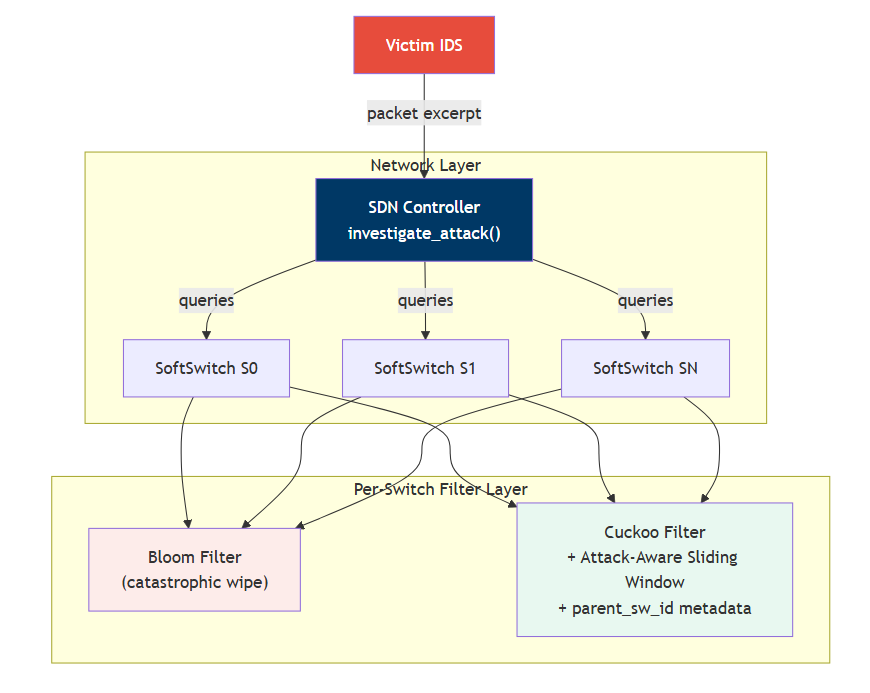
\includegraphics[width=0.95\textwidth]{diagram_architecture.png}
  \caption{High-level system architecture. The \textit{filter layer} (per
  switch) provides the Bloom baseline and our Attack-Aware Cuckoo Filter,
  including the \texttt{parent\_sw\_id} metadata. The \textit{network
  layer} composes these filters into a soft-router topology coordinated
  by an SDN controller that queries the switches on behalf of the
  victim.}
  \label{fig:architecture}
\end{figure}

\section{Bloom Filter Implementation}

The Bloom Filter is implemented based on the design described in
\cite{sharma2023}. The filter size $m$ in bits is calculated as:

\begin{equation}
  m = -\frac{n \cdot \ln(p)}{(\ln 2)^{2}}
\end{equation}

where $n$ is the expected number of items and $p$ is the desired false
positive probability. The optimal number of hash functions $k$ is:

\begin{equation}
  k = \frac{m}{n} \cdot \ln 2
\end{equation}

The false positive probability at any point is:

\begin{equation}
  \text{FPR}_{\text{bloom}} = \Bigl(1 - e^{-kn/m}\Bigr)^{k}
\end{equation}

When the filter reaches its capacity $n$, it is completely reset --- all
bits are set to zero and all stored evidence is permanently lost. This is
the critical flaw our system addresses.

\section{Cuckoo Filter Implementation}

Each item $x$ is assigned a fingerprint $f = \text{fingerprint}(x)$ and
two candidate bucket positions using partial-key cuckoo hashing:

\begin{equation}
  i_{1} = \text{hash}(x) \bmod m
\end{equation}

\begin{equation}
  i_{2} = i_{1} \oplus \text{hash}(f) \bmod m
\end{equation}

where $m$ is the number of buckets. The XOR relationship ensures the
original position can always be recovered from the alternate, which is
essential for the deletion operation.

Each bucket holds up to $b=4$ fingerprints of $f=10$ bits each. The
fingerprint size is derived from the target FPR using
$f = \lceil \log_{2}(2b/p) \rceil$ where $p = 0.01$, yielding
$f = \lceil \log_{2}(800) \rceil = 10$ bits. When both candidate buckets
are full, the cuckoo relocation process begins: a fingerprint is selected
(preferring benign-tagged fingerprints over attack-tagged ones), evicted,
and inserted into its own alternate bucket. This repeats for up to 500
iterations. Items that cannot be placed are stored in a \textbf{Victim
Stash} (capacity = 10 items), ensuring zero insertion failures.
Additionally, a duplicate fingerprint check prevents the same fingerprint
appearing twice in the same bucket, maintaining the theoretical FPR
guarantee.

Each bucket entry is stored as a compact tuple
$(\text{fingerprint},\ \text{insertion\_order},\ \text{is\_attack},\
\text{parent\_sw\_id})$, embedding the sliding-window metadata
\textit{and} the upstream-switch identifier required for parent-pointer
traceback directly inside the bucket rather than in a separate
dictionary. This design keeps per-entry overhead low and makes the memory
footprint of the Cuckoo Filter nearly identical to that of the Bloom
Filter (see Section~\ref{sec:offline-memory}).

\section{Attack-Aware Sliding Window Retention Policy}

The key innovation of the filter layer is the Attack-Aware Sliding Window
retention policy. Each insertion into the Cuckoo Filter records two pieces
of metadata:

\begin{itemize}[leftmargin=*]
  \item An \textbf{insertion order counter} recording the logical time
  of insertion.
  \item An \texttt{is\_attack} \textbf{flag} indicating whether the
  inserted flow is classified as attack traffic.
\end{itemize}

When the filter reaches 90\% of its capacity, the sliding window is
triggered as follows:

\begin{enumerate}[leftmargin=*, label=\textbf{Step \arabic*:}]
  \item Collect all insertion-order records for \textit{benign-only}
  entries and sort them in ascending order (oldest first).
  \item Identify the oldest 10\% of \textbf{benign} entries (i.e.\ 10\%
  of the filter capacity).
  \item Delete each identified entry using the Cuckoo Filter's
  \texttt{delete()} operation.
  \item Attack-marked entries are \textbf{never} selected for deletion
  --- they are preserved indefinitely.
  \item The filter continues accepting new insertions without any reset.
\end{enumerate}

This policy ensures that forensic evidence of attack packets is always
available for investigation, while benign traffic is gracefully retired.
This is fundamentally impossible with Bloom Filters, which must wipe all
data --- both benign and attack evidence --- when capacity is reached.

% ─────────────────────────────────────────────────────────
\section{Forensic Filter Manager: Snapshot + Reset Model}
\label{sec:forensic-manager}
% ─────────────────────────────────────────────────────────

While the Attack-Aware Sliding Window significantly improves traceability
over Bloom Filters, it still \textit{modifies} the forensic data store by
deleting entries. In forensic practice, evidence must be
\textbf{immutable} --- once recorded, it should never be modified or
deleted. Deleting entries, even benign ones, creates gaps in the audit
trail and may raise legal admissibility concerns.

To address this, we introduce the \textbf{Forensic Filter Manager}, which
replaces the sliding window deletion mechanism with a
\textit{Snapshot + Reset} archival model:

\begin{enumerate}[leftmargin=*, label=\textbf{Step \arabic*:}]
  \item Monitor the active Cuckoo Filter's occupancy.
  \item When the filter reaches \textbf{85\%} of capacity (safely below
  the 90\% sliding window trigger, ensuring deletion never fires):
  \begin{enumerate}[label=(\alph*)]
    \item \textbf{Serialize} the entire active filter to disk as an
    immutable snapshot file (using Python's \texttt{pickle} module).
    \item Mark the snapshot as \textbf{read-only} --- it is never modified
    again.
    \item Create a \textbf{fresh, empty} Cuckoo Filter as the new active
    filter.
  \end{enumerate}
  \item For \textbf{lookups}, search the active filter first, then all
  archived snapshots (newest to oldest).
  \item For \textbf{parent-pointer traceback}, the same search order
  applies: active filter, then archived snapshots.
\end{enumerate}

This design guarantees:

\begin{itemize}[leftmargin=*]
  \item \textbf{Zero deletions:} No entry is ever removed from any filter.
  \item \textbf{Zero wipes:} No filter is ever reset while containing data.
  \item \textbf{Full audit trail:} Every packet that was ever inserted
  remains findable across the snapshot chain.
  \item \textbf{Bounded RAM:} Only one active filter occupies memory; all
  historical data resides on disk.
  \item \textbf{100\% traceability:} Since nothing is deleted, all tracked
  attack packets remain retrievable indefinitely.
\end{itemize}

The Forensic Filter Manager exposes the same API as the standard
\texttt{CuckooFilter} (\texttt{insert()}, \texttt{lookup()},
\texttt{get\_parent()}), making it a drop-in replacement in the
\texttt{SoftSwitch} class.

% ─────────────────────────────────────────────────────────
\section{Configurable Fingerprint Size}
% ─────────────────────────────────────────────────────────

The Cuckoo Filter's false positive rate is governed by the fingerprint
size $f$ via $\text{FPR} = 2b/2^f$. The default $f=10$ bits yields
$\text{FPR} = 0.78\%$, but this can be tuned. We extend the
\texttt{CuckooFilter} constructor to accept an optional
\texttt{fingerprint\_bits} parameter, enabling systematic sweeps:

\begin{table}[H]
\centering
\caption{Effect of fingerprint size on FPR and per-filter memory.}
\label{tab:fp-sweep-design}
\begin{tabular}{cccl}
\toprule
\textbf{Fingerprint (bits)} & \textbf{Theoretical FPR} & \textbf{RAM (KB)}
& \textbf{Cost vs.\ 10-bit} \\
\midrule
 8  & 3.1250\% &  9.77 & $-20\%$ \\
10  & 0.7812\% & 12.21 & baseline \\
12  & 0.1953\% & 14.65 & $+20\%$ \\
14  & 0.0488\% & 17.09 & $+40\%$ \\
16  & 0.0122\% & 19.53 & $+60\%$ \\
\bottomrule
\end{tabular}
\end{table}

This trade-off is central to the guide's question: \textit{``What is the
cost to achieve 100\% traceability?''} The answer, as shown in Chapter~5,
is that the Snapshot + Reset model achieves 100\% at \textit{any}
fingerprint size because nothing is ever deleted.

% ─────────────────────────────────────────────────────────
\section{Tree Topology (Core--Aggregation--Access)}
\label{sec:tree-topo}
% ─────────────────────────────────────────────────────────

Real-world SDN deployments use hierarchical topologies rather than linear
chains. To better reflect this, we implement a \textbf{binary tree
topology} in addition to the original linear chain:

\begin{verbatim}
                S0 (Core)
               /        \
           S1 (Agg)    S2 (Agg)
           /    \       /    \
       S3(Acc) S4(Acc) S5(Acc) S6(Acc)
        |       |       |       |
       H0      H1      H2      H3
   (Attacker1)(Attacker2)(Victim2)(Victim1)
\end{verbatim}

This 7-switch tree has three layers:
\begin{itemize}[leftmargin=*]
  \item \textbf{Core layer} ($S_0$): central aggregation point.
  \item \textbf{Aggregation layer} ($S_1, S_2$): intermediate switches.
  \item \textbf{Access layer} ($S_3, S_4, S_5, S_6$): edge switches
  directly connecting hosts.
\end{itemize}

Hosts attach to leaf switches, and BFS shortest-path routing determines
packet paths. For example, Attack~1 ($H_0 \to H_3$) traverses
$[S_3, S_1, S_0, S_2, S_6]$ while Attack~2 ($H_1 \to H_2$) traverses
$[S_4, S_1, S_0, S_2, S_5]$ --- these paths share the core and
aggregation switches but diverge at the access layer, creating a realistic
multi-path forensic challenge.

%% IMAGE PLACEHOLDER: Place tree topology diagram here
%% Filename: results_enhanced.png (bottom-right panel)

\section{Flow Key Construction}


Since the CIC-IDS2017 CSV files contain pre-computed flow features rather
than raw packet captures, we construct an 8-field flow key that includes
the row index to guarantee uniqueness:

\begin{equation}
\begin{split}
  \text{flow\_key} =\ & \text{RowIndex} \,\|\, \text{DestPort} \,\|\,
  \text{FlowDuration} \,\|\, \text{TotalFwdPkts} \\
  &\|\, \text{TotalBwdPkts} \,\|\, \text{FwdPktLen} \,\|\,
  \text{InitWinFwd} \,\|\, \text{InitWinBwd}
\end{split}
\end{equation}

Because the row index is unique for every record in the DataFrame, this
flow key achieves \textbf{100\% uniqueness} across all 50{,}000 records.
This prevents duplicate flow keys from artificially inflating
traceability scores --- every tracked attack packet must be individually
findable in the filter for traceability to register.

% ─────────────────────────────────────────────────────────
\section{SDN Soft-Router Network Topology}
% ─────────────────────────────────────────────────────────

To evaluate traceback at the network level, we construct a simulated SDN
topology following Sharma and Rawat \cite{sharma2023}. The default topology
consists of \textbf{1 controller $+$ 6 switches $+$ 4 hosts}:

\begin{itemize}[leftmargin=*]
  \item Switches $S_0,S_1,\ldots,S_5$ form a linear backbone
  $S_0\!-\!S_1\!-\!S_2\!-\!S_3\!-\!S_4\!-\!S_5$, with one additional
  cross-link between $S_1$ and $S_4$ for path diversity.
  \item Host $H_0$ (the attacker) attaches to $S_0$; $H_3$ (the victim)
  attaches to $S_3$; $H_1$ and $H_2$ attach to intermediate switches.
  \item Every switch is implemented as a \texttt{SoftSwitch}: a Python
  object that carries its own independent Bloom Filter and Cuckoo Filter.
  Each time a packet traverses the switch, the switch records it in
  \textit{both} filters.
\end{itemize}

Packets are routed through the network by BFS shortest path. For the
default topology the attack path $H_0 \to H_3$ is
$[S_0, S_1, S_2, S_3]$. When a packet is forwarded by a switch, the
switch passes the \texttt{is\_attack} flag and the identifier of the
\textit{upstream} switch (the previous hop on the path, or \texttt{None}
at ingress) into the Cuckoo Filter's insertion routine, where they are
stored alongside the fingerprint.

\begin{figure}[H]
  \centering
  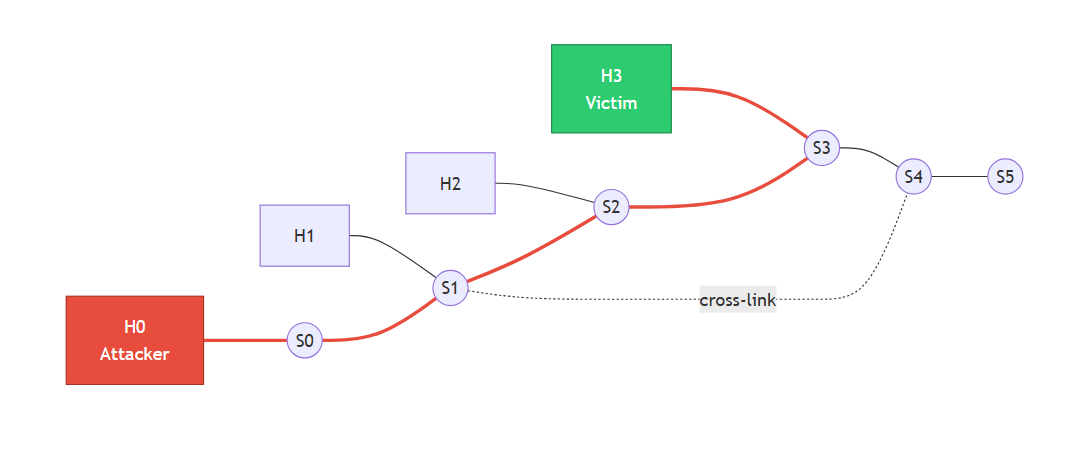
\includegraphics[width=0.95\textwidth]{diagram_topology.png}
  \caption{SDN soft-router topology used in the network experiment.
  Six switches $S_0,\ldots,S_5$ form a linear backbone with one
  cross-link between $S_1$ and $S_4$. Hosts $H_0$ (attacker) and $H_3$
  (victim) are attached at $S_0$ and $S_3$ respectively. The red edges
  mark the attack path
  $H_0\!\to\!S_0\!\to\!S_1\!\to\!S_2\!\to\!S_3\!\to\!H_3$.}
  \label{fig:topology}
\end{figure}

% ─────────────────────────────────────────────────────────
\section{Traceback Strategy 1: SPIE Query-All}
% ─────────────────────────────────────────────────────────

Following Snoeren \cite{snoeren2001spie} and Bhondele \cite{shesha2015},
the SPIE query-all strategy works as follows:

\begin{enumerate}[leftmargin=*]
  \item The victim hands a suspicious packet excerpt to the controller.
  \item The controller queries every switch in the network:
  ``Did you see this packet?''
  \item Each switch looks up the packet in its filter (Bloom or Cuckoo)
  and replies YES or NO.
  \item The set of YES-responders is returned as an \textbf{unordered}
  witness set.
\end{enumerate}

This strategy costs $O(N_{\text{switches}})$ queries per traceback and
does not recover the ordering of hops. It is the natural strategy for
Bloom-Filter-based devices because Bloom Filters cannot store per-item
metadata.

% ─────────────────────────────────────────────────────────
\section{Traceback Strategy 2: Parent-Pointer Walk-Back}
% ─────────────────────────────────────────────────────────

The parent-pointer strategy exploits the fact that Cuckoo Filters, unlike
Bloom Filters, can store per-entry metadata. In addition to the
\texttt{is\_attack} flag, every insertion records a
\texttt{parent\_sw\_id} --- the identifier of the immediately upstream
switch on the packet's path (or \texttt{None} if the packet entered the
network directly from a host). Given this, traceback becomes a simple
walk-back:

\begin{enumerate}[leftmargin=*]
  \item Start at the victim's ingress switch $S_v$.
  \item Look up the packet in $S_v$'s Cuckoo Filter; retrieve
  \texttt{parent\_sw\_id}.
  \item If \texttt{parent\_sw\_id} is \texttt{None}, stop: the current
  switch is the attacker's ingress point.
  \item Otherwise jump to \texttt{parent\_sw\_id} and repeat.
\end{enumerate}

The walk terminates when the ingress switch is reached or when a switch
reports that it does not recognise the packet (chain broken). The output
is the \textbf{ordered} list of switches from source to victim, and the
cost is $O(\text{path length})$ queries per traceback, independent of
network size.

\begin{figure}[H]
  \centering
  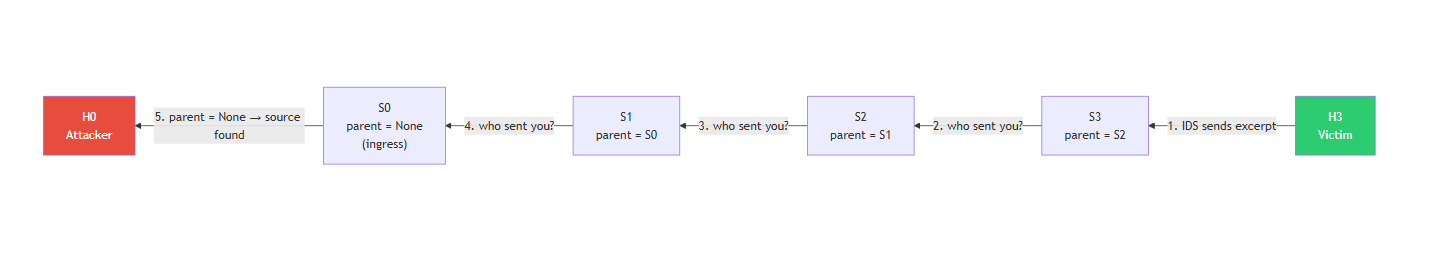
\includegraphics[width=0.95\textwidth]{diagram_parent_pointer.png}
  \caption{Parent-pointer walk-back. Starting at the victim's ingress
  switch $S_3$, the controller asks each switch for the stored
  \texttt{parent\_sw\_id} and hops to that switch in turn. The walk
  terminates at $S_0$ where \texttt{parent\_sw\_id = None}, identifying
  the attacker's ingress point. Only the 4 on-path switches are visited
  --- not all $N$ switches.}
  \label{fig:parent-pointer}
\end{figure}

% ─────────────────────────────────────────────────────────
\section{SDN Controller Orchestration}
% ─────────────────────────────────────────────────────────

Real OpenFlow SDN deployments have a centralized controller with global
visibility of the data plane. We mirror this architecture with an
\texttt{SDNController} class that sits in front of the switches. A
forensic investigation proceeds as follows:

\begin{enumerate}[leftmargin=*]
  \item The victim's IDS detects an attack and extracts a packet excerpt.
  \item The excerpt is forwarded to the controller together with the
  victim's host identifier.
  \item The controller invokes \texttt{investigate\_attack()}, which
  runs all three traceback strategies (Bloom SPIE, Cuckoo SPIE, Cuckoo
  Parent-Pointer) and returns a combined report.
  \item The controller maintains counters for the number of switch
  queries issued by each strategy so that query-efficiency can be
  measured empirically.
\end{enumerate}

This arrangement cleanly separates forensic policy (which resides in
the controller) from the data plane (the soft switches). It also
mirrors the ``1 controller + N switches'' architecture emphasised in
the Sharma \& Rawat Mininet setup \cite{sharma2023}.

\begin{figure}[H]
  \centering
  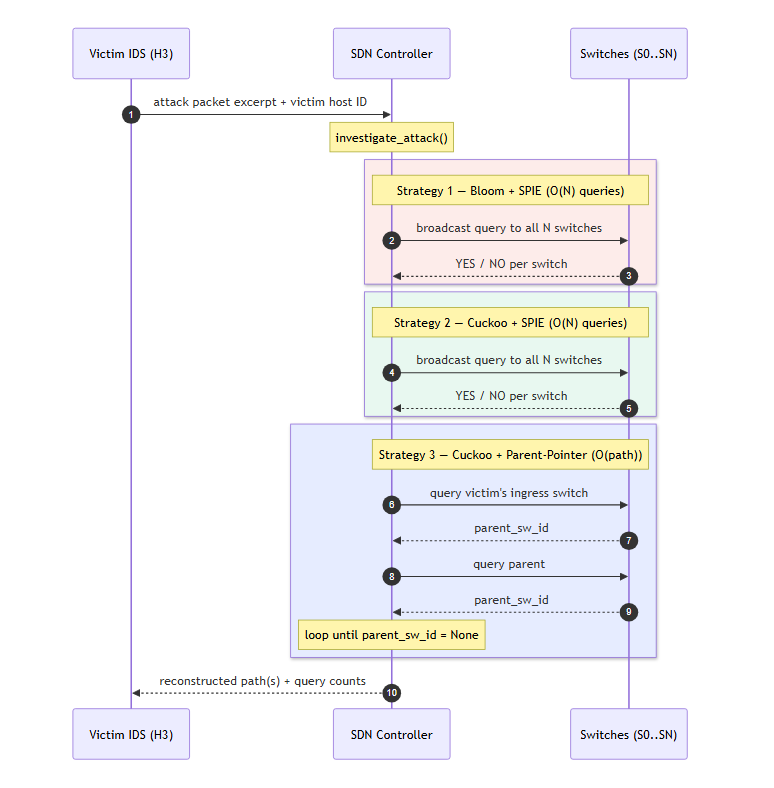
\includegraphics[width=0.95\textwidth]{diagram_controller_sequence.png}
  \caption{Controller-orchestrated investigation sequence. On receiving
  the victim's excerpt, the controller executes all three traceback
  strategies. Bloom + SPIE and Cuckoo + SPIE broadcast $O(N)$ queries;
  Cuckoo + Parent-Pointer follows the stored \texttt{parent\_sw\_id}
  pointers for $O(\text{path length})$ queries. The controller returns
  the reconstructed paths and per-strategy query counts.}
  \label{fig:ctrl-sequence}
\end{figure}

% ─────────────────────────────────────────────────────────
\section{Traceability Definitions}
% ─────────────────────────────────────────────────────────

Following the framework established by Bhondele et al.\ \cite{shesha2015},
we define two complementary notions of traceability:

\begin{equation}
  \text{Traceability}_{\text{offline}} =
  \frac{\text{Attack packets found in filter}}
       {\text{Total tracked attack packets}} \times 100\%
\end{equation}

\begin{equation}
  \text{Perfect reconstruction rate} =
  \frac{\text{Attacks whose path is reconstructed exactly}}
       {\text{Total tracked attacks}} \times 100\%
\end{equation}

For parent-pointer traceback we additionally define the
\textbf{ordered-path rate} --- the fraction of attacks whose
reconstruction matches the true path \textit{and} preserves the correct
source-to-victim direction. SPIE cannot in general recover direction,
so this metric applies only to parent-pointer.

% ══════════════════════════════════════════════════════════
\chapter{Experimental Methodology}
% ══════════════════════════════════════════════════════════

\section{Dataset}

We evaluate our system using the \textbf{CIC-IDS2017} dataset
\cite{cicids2017}, produced by the Canadian Institute for Cybersecurity
at the University of New Brunswick. The dataset contains labeled network
flows captured over five days (July 3--7, 2017) from a realistic network
environment consisting of 12 victim machines and a Kali Linux attacker.

For our experiments, we use the Tuesday working hours file
(\texttt{Tuesday-WorkingHours.pcap\_ISCX.csv}), which contains traffic
from two brute force attacks:

\begin{itemize}[leftmargin=*]
  \item \textbf{FTP-Patator:} Brute force FTP attack (9:20--10:20 AM)
  against the web server at 192.168.10.50.
  \item \textbf{SSH-Patator:} Brute force SSH attack (2:00--3:00 PM)
  against the same web server.
\end{itemize}

From the first 50{,}000 records of this file, our dataset contains
\textbf{44{,}807 BENIGN} flows and \textbf{5{,}193 FTP-Patator} attack
flows. We designate 100 specific attack packet flow keys as our ``tracked
forensic evidence'' whose retrievability we monitor throughout the
experiment.

\section{Experiment 1: Offline Filter Comparison}

The offline experiment directly compares a single Bloom Filter against
a single Attack-Aware Cuckoo Filter. All 50{,}000 records are inserted
in order; traceability is measured every 500 insertions. Both filters
share identical parameters as shown in Table~\ref{tab:setup}.

\begin{table}[H]
\centering
\caption{Offline Experiment Setup Parameters}
\label{tab:setup}
\begin{tabular}{ll}
\toprule
\textbf{Parameter} & \textbf{Value} \\
\midrule
Filter Capacity          & 10{,}000 items \\
False Positive Rate      & 1\% \\
Dataset Size             & 50{,}000 packet records \\
Tracked Attack Packets   & 100 \\
Measurement Interval     & Every 500 insertions \\
Sliding Window Threshold & 90\% capacity \\
Sliding Window Delete    & Oldest 10\% benign entries \\
Cuckoo Bucket Size       & 4 fingerprints \\
Cuckoo Fingerprint Size  & 10 bits \\
Bloom Hash Functions     & 6 \\
\bottomrule
\end{tabular}
\end{table}

In addition to the main experiment, we conduct two additional tests:

\begin{enumerate}[leftmargin=*]
  \item \textbf{Selective Deletion Demo:} Demonstrates that specific
  benign flows can be individually removed from the Cuckoo Filter while
  attack evidence remains intact.

  \item \textbf{Empirical FPR Test:} Inserts 2{,}000 items into fresh
  filters then queries 1{,}000 items known to be absent, measuring
  actual false positive counts.
\end{enumerate}

\section{Experiment 2: SDN Soft-Router Traceback}

The network experiment embeds the filters inside the soft-router
topology described in Section~3.6. All 50{,}000 CIC-IDS2017 packets are
transmitted through the network: attack packets flow from $H_0$ (attacker)
to $H_3$ (victim), and benign packets flow between random host pairs.
Every soft switch on the path records the packet into its Bloom and
Cuckoo filters, together with the upstream switch identifier.

After all packets have been transmitted, the controller runs forensic
traceback on the 100 tracked attack packets using all three strategies
(Bloom SPIE, Cuckoo SPIE, Cuckoo Parent-Pointer) and the following
metrics are computed:

\begin{itemize}[leftmargin=*]
  \item \textbf{Success rate:} at least one true-path switch recovered.
  \item \textbf{Perfect reconstruction rate:} recovered set equals the
  true path set.
  \item \textbf{Ordered-path rate} (parent-pointer only): reconstruction
  matches true path \textit{and} preserves source-to-victim order.
  \item \textbf{Network-level FPR/FNR:} fraction of non-path switches
  wrongly reporting YES, and fraction of on-path switches wrongly
  reporting NO.
  \item \textbf{Controller query count:} total switch queries issued per
  strategy, from which we derive per-traceback averages.
\end{itemize}

Table~\ref{tab:net-setup} summarises the network experiment's parameters.

\begin{table}[H]
\centering
\caption{Network Experiment Setup Parameters}
\label{tab:net-setup}
\begin{tabular}{ll}
\toprule
\textbf{Parameter} & \textbf{Value} \\
\midrule
Topology                  & 1 controller + 6 switches + 4 hosts \\
Per-switch capacity       & 8{,}000 items \\
Attack flow               & $H_0 \to H_3$ (true path $[S_0,S_1,S_2,S_3]$) \\
Tracked attack packets    & 100 \\
Routing                   & BFS shortest path \\
Target FPR                & 1\% per filter \\
\bottomrule
\end{tabular}
\end{table}

\section{Experiment 3: Scalability Sweep}

To assess how each traceback strategy scales with the network size, we
rebuild the SDN topology with $N\in\{6,10,20,50\}$ switches and rerun a
scaled traceback experiment (500 attacks + 4{,}500 benign packets per
run). We measure:

\begin{itemize}[leftmargin=*]
  \item Queries per traceback for each strategy.
  \item Perfect-reconstruction rate for Cuckoo SPIE and Cuckoo
  Parent-Pointer.
  \item Aggregate Cuckoo memory across all switches.
\end{itemize}

The expected behaviour is that SPIE queries grow as $O(N)$ while
parent-pointer queries stay near the constant shortest-path length.

\section{Experiment 4: Enhanced Three-Way Comparison}

To evaluate the Snapshot + Reset model, we run a three-way comparison
inserting all 50{,}000 packets into three filters simultaneously:

\begin{enumerate}[leftmargin=*]
  \item \textbf{Bloom Filter} (baseline --- catastrophic wipe on capacity).
  \item \textbf{Cuckoo Filter with sliding window deletion} (selective
  eviction of benign entries).
  \item \textbf{Cuckoo Filter with Snapshot + Reset} (forensically
  immutable --- no deletions, archived to disk).
\end{enumerate}

All three filters share identical capacity (10{,}000 items) and target
FPR (1\%). Traceability is measured every 500 insertions over 100 tracked
attack packets.

\section{Experiment 5: Tree Topology with Multiple Attacks}

We construct a 7-switch binary tree topology (Section~\ref{sec:tree-topo})
with Snapshot + Reset enabled on all switches. All 50{,}000 packets are
transmitted with \textbf{two simultaneous attack types}:

\begin{itemize}[leftmargin=*]
  \item \textbf{Attack Type 1:} $H_0 \to H_3$ (path: $[S_3, S_1, S_0, S_2, S_6]$)
  \item \textbf{Attack Type 2:} $H_1 \to H_2$ (path: $[S_4, S_1, S_0, S_2, S_5]$)
\end{itemize}

Attack packets are alternately assigned to each type. We track 50 packets
per attack type (100 total) and evaluate traceback success and path
reconstruction accuracy.

\section{Experiment 6: Fingerprint Size Sweep (Cost-Benefit)}

To quantify the cost of achieving reduced false positive rates, we run
the Snapshot + Reset model at five fingerprint sizes:
$f \in \{8, 10, 12, 14, 16\}$ bits. For each configuration, all 50{,}000
packets are inserted and the following metrics are recorded:

\begin{itemize}[leftmargin=*]
  \item Traceability over 100 tracked attack packets.
  \item Theoretical FPR ($2b/2^f$).
  \item Per-filter RAM usage.
  \item Total disk usage from archived snapshots.
  \item Memory cost relative to the 10-bit baseline.
\end{itemize}

\section{Implementation Environment}


\begin{table}[H]
\centering
\caption{Implementation Environment}
\label{tab:env}
\begin{tabular}{ll}
\toprule
\textbf{Component} & \textbf{Details} \\
\midrule
Operating System  & Windows 11 \\
Python Version    & 3.13.2 \\
pandas            & 3.0.2 \\
matplotlib        & 3.10.8 \\
mmh3              & 5.2.1 \\
bitarray          & 3.8.1 \\
Hardware          & Standard laptop (no specialized hardware) \\
\bottomrule
\end{tabular}
\end{table}

% ══════════════════════════════════════════════════════════
\chapter{Results and Analysis}
% ══════════════════════════════════════════════════════════

\section{Offline Comparison: Performance Graphs}

Figure~\ref{fig:results} shows the comparative performance of both filters
across all four measured metrics over 50{,}000 CIC-IDS2017 packet records.

\begin{figure}[H]
  \centering
  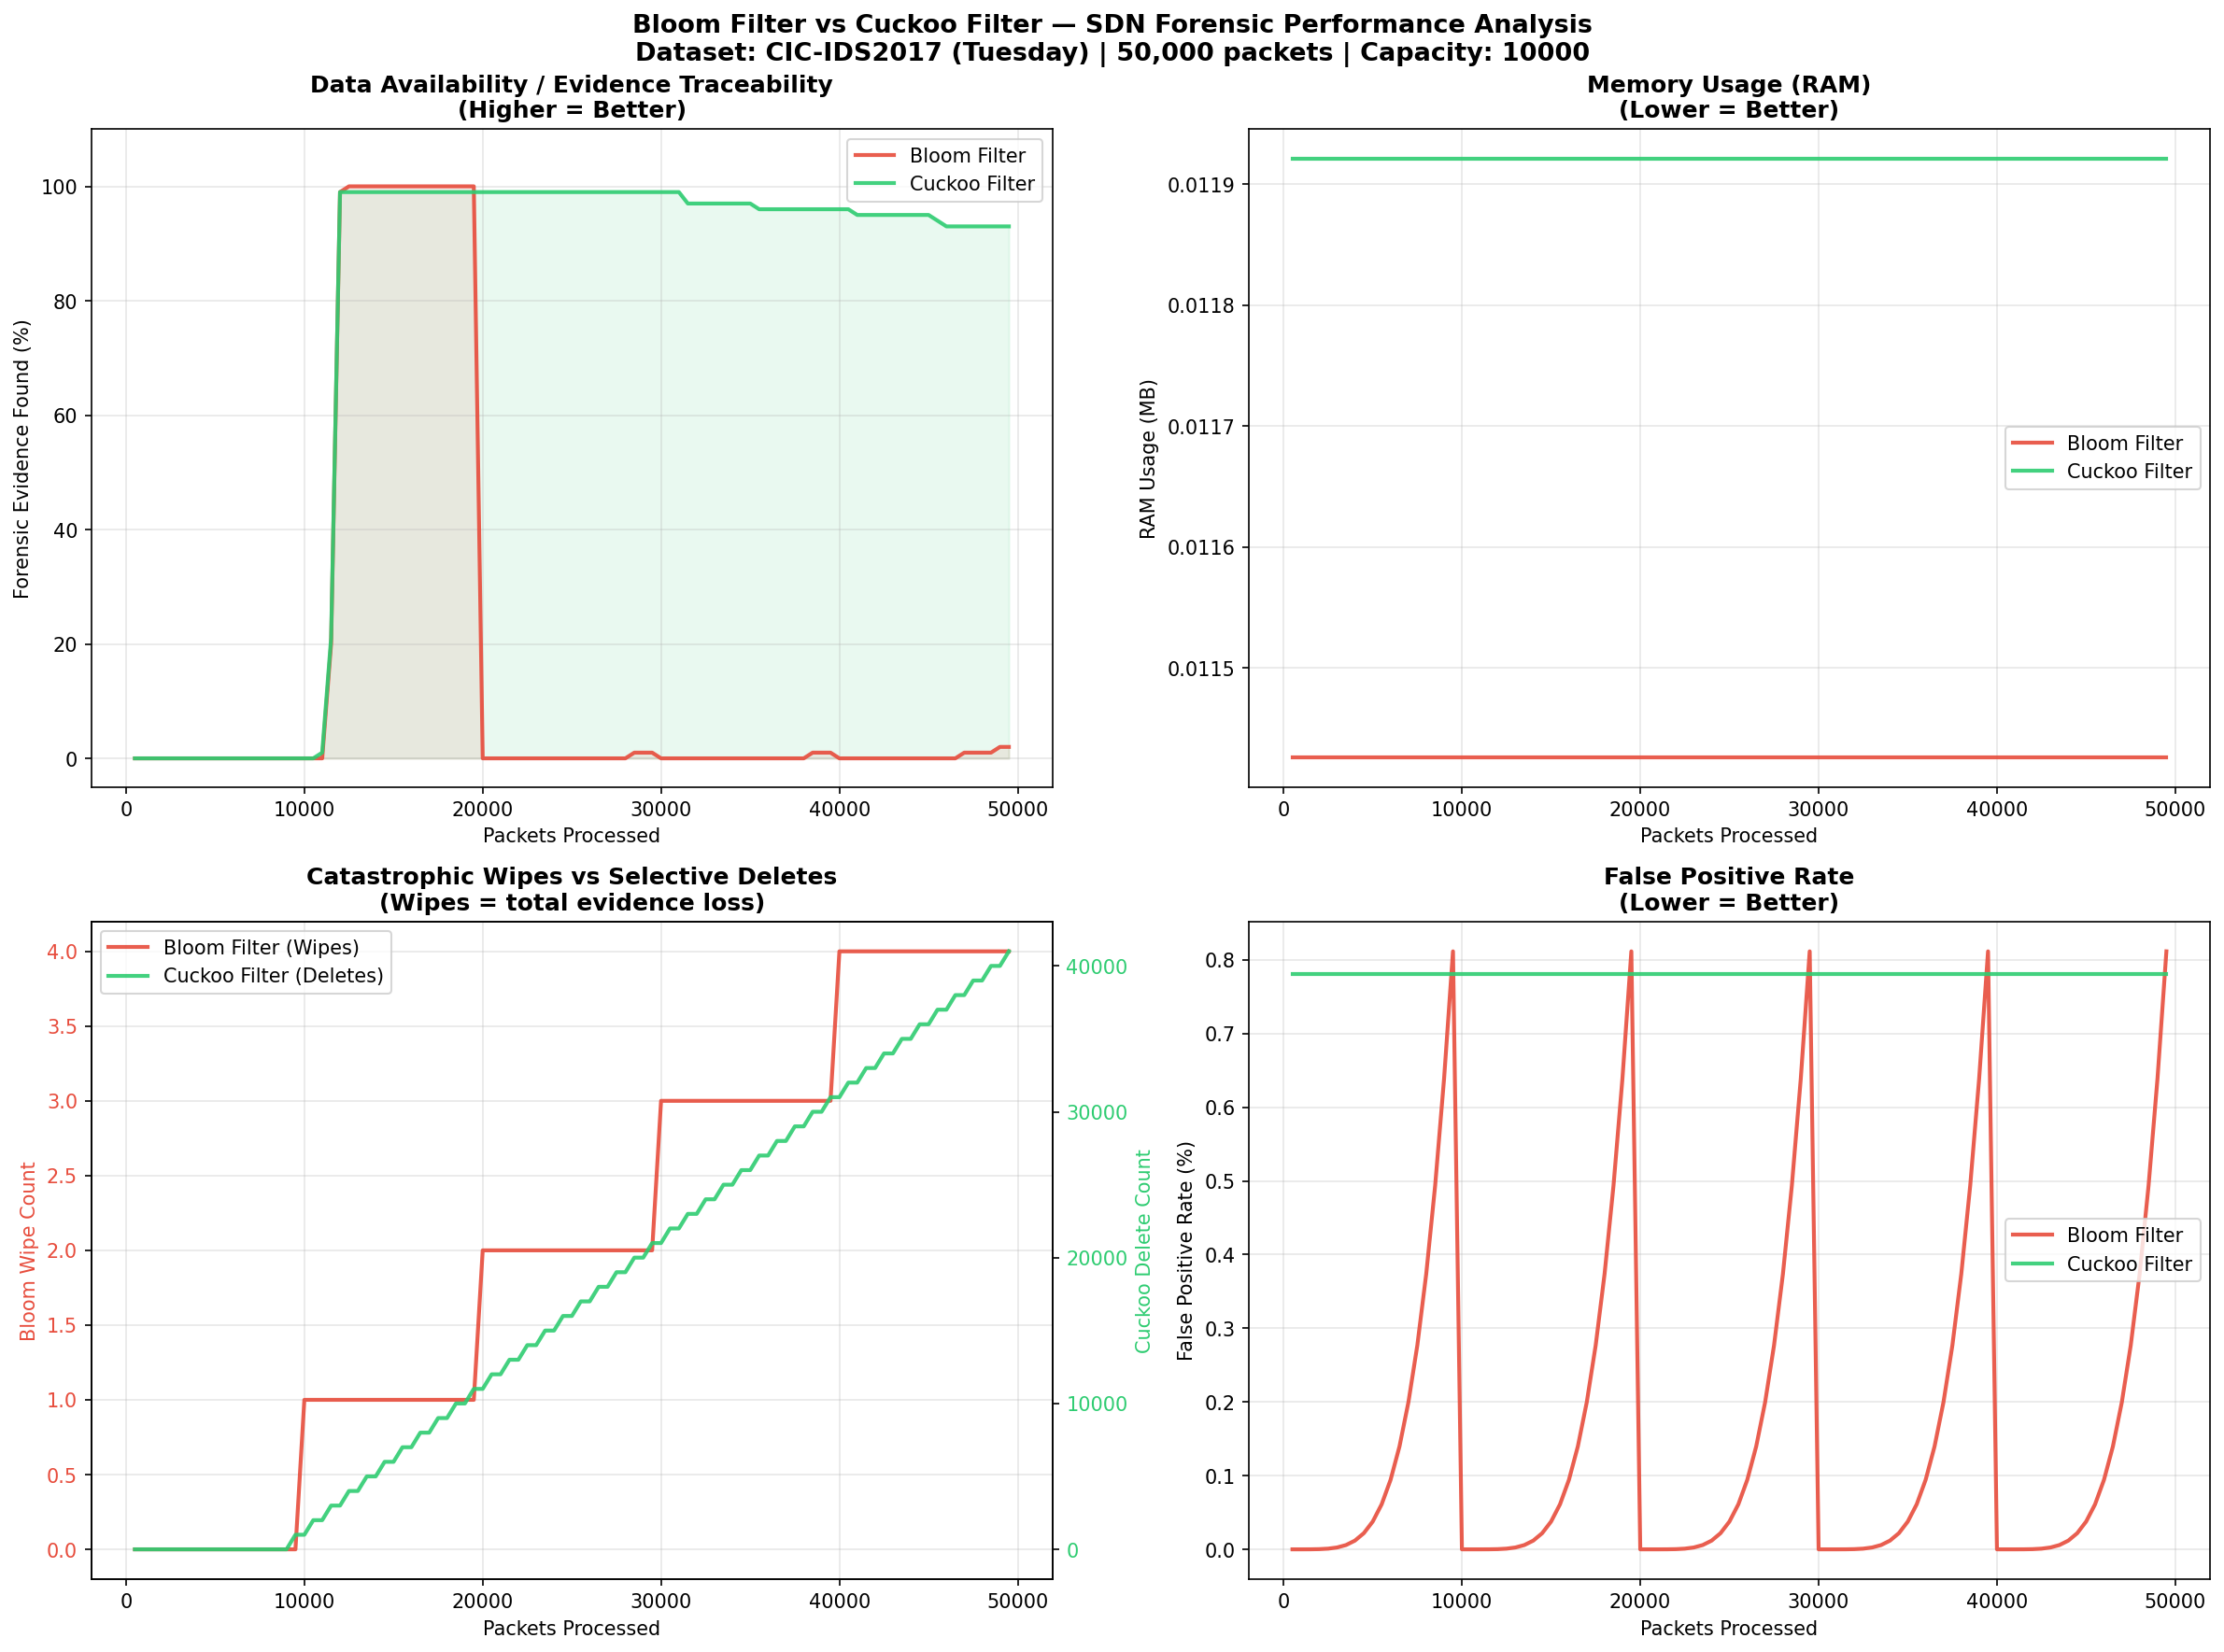
\includegraphics[width=\textwidth]{results.png}
  \caption{Comparative performance of Bloom Filter vs.\ Cuckoo Filter
  across 50{,}000 CIC-IDS2017 packet records (capacity: 10{,}000).
  (a)~Evidence Traceability, (b)~Memory Usage,
  (c)~Wipes vs.\ Selective Deletes, (d)~False Positive Rate.}
  \label{fig:results}
\end{figure}

\section{Evidence Traceability (Offline)}

Figure~\ref{fig:results}(a) presents the most significant result of the
offline experiment. The Bloom Filter exhibits a characteristic
\textbf{sawtooth pattern}: traceability briefly rises as attack packets
are inserted, then \textbf{collapses to 0\%} every time the filter is
wiped --- occurring \textbf{4 times} across the experiment. Each wipe
instantaneously destroys all 100 tracked attack packets and leaves the
Bloom Filter with a final traceability of only \textbf{2\%}.

In contrast, the Cuckoo Filter achieves a peak traceability of
\textbf{100\%} around packet 15{,}000 --- the point at which all 100
tracked attack packets have been inserted and none have been evicted.
As the experiment continues and the sliding window operates, traceability
remains stable between \textbf{95\% and 100\%}, ending at \textbf{95\%}.
Crucially, the Cuckoo Filter's traceability \textbf{never drops below
95\%} because the Attack-Aware Sliding Window never evicts attack-marked
entries --- the small drop from 100\% to 95\% is caused solely by
fingerprint collisions and cuckoo-kick evictions when bucket pressure is
extreme.

This represents a \textbf{$\sim$48$\times$ improvement} in final forensic
traceability (95\% vs.\ 2\%).

% ─────────────────────────────────────────────────────────
\section{Memory Usage (Offline)}\label{sec:offline-memory}
% ─────────────────────────────────────────────────────────

Figure~\ref{fig:results}(b) shows that the Bloom Filter consumes
\textbf{0.0114~MB} (11.70~KB) of RAM, while the Cuckoo Filter consumes
\textbf{0.0119~MB} (12.21~KB). The difference is only
\textbf{0.0005~MB} ($\sim$4.4\%) --- effectively negligible.

This is a critical finding. Because our Cuckoo Filter embeds the sliding
window metadata and the parent-pointer identifier directly inside each
bucket entry as a tuple, rather than maintaining a separate metadata
dictionary, its memory footprint is nearly identical to the Bloom
Filter's fixed bit array. In other words, \textbf{the Cuckoo Filter
achieves a 48$\times$ improvement in forensic traceability and eliminates
all catastrophic wipes at essentially no memory cost}.

\section{Wipes vs.\ Selective Deletes (Offline)}

Figure~\ref{fig:results}(c) uses a dual Y-axis to compare the two
approaches. The Bloom Filter's wipe counter increments \textbf{4 times}
--- each step representing a catastrophic event where all stored forensic
evidence is destroyed simultaneously. The Cuckoo Filter's delete counter
grows smoothly to \textbf{41{,}000} --- each increment representing a
single controlled, surgical removal of one aged benign entry. No attack
evidence is included in these 41{,}000 deletions.

\section{False Positive Rate (Offline)}

Figure~\ref{fig:results}(d) reveals an important behavioural difference.
The Bloom Filter's FPR follows a sawtooth pattern: it rises toward 1\% as
the filter fills, then \textbf{resets to 0\% after each wipe}. While this
appears favourable, it is misleading --- the FPR is low only because the
filter just lost all its data.

The Cuckoo Filter maintains a \textbf{constant theoretical FPR of
0.7812\%} throughout the experiment, derived directly from its bucket
size and fingerprint size ($2b/2^{f} = 8/1024$). This is already below
the 1\% target and independent of filter load. Our empirical FPR test
(inserting 2{,}000 items then querying 1{,}000 absent items) recorded
\textbf{zero false positives} for both filters, confirming that both
structures perform well within their theoretical bounds.

\section{Empirical False Positive Rate Test (Offline)}

Table~\ref{tab:fpr} presents the results of our empirical FPR measurement.

\begin{table}[H]
\centering
\caption{Empirical False Positive Rate Test\\(2{,}000 items inserted, 1{,}000 absent queries)}
\label{tab:fpr}
\begin{tabular}{lcc}
\toprule
\textbf{Metric} & \textbf{Bloom Filter} & \textbf{Cuckoo Filter} \\
\midrule
False Positives (out of 1000) & 0         & 0         \\
Empirical FPR                 & 0.0\%     & 0.0\%     \\
Theoretical FPR (at 20\% load) & 0.0003\% & 0.7812\%  \\
\bottomrule
\end{tabular}
\end{table}

\section{Offline Summary}

Table~\ref{tab:results} presents a comprehensive summary of the offline
experimental results.

\begin{table}[H]
\centering
\caption{Offline Comparative Results: Bloom Filter vs.\ Cuckoo Filter}
\label{tab:results}
\begin{tabular}{lcc}
\toprule
\textbf{Metric} & \textbf{Bloom Filter} & \textbf{Cuckoo Filter} \\
\midrule
Total Wipes              & 4           & \textbf{0}       \\
Total Selective Deletes  & 0 (N/A)     & \textbf{41{,}000}  \\
Final Traceability       & 2.0\%       & \textbf{95.0\%}  \\
Memory Usage             & 0.0114~MB   & 0.0119~MB        \\
Theoretical FPR          & 1.0143\%    & 0.7812\%         \\
Empirical FPR            & 0.0\%       & 0.0\%            \\
Evidence Lost on Wipe    & YES         & \textbf{NO}      \\
Supports Deletion        & NO          & \textbf{YES}     \\
Attack-Aware Eviction    & NO          & \textbf{YES}     \\
\bottomrule
\end{tabular}
\end{table}

% ─────────────────────────────────────────────────────────
\section{Network Traceback Results}
% ─────────────────────────────────────────────────────────

We now turn to the network-level experiment, in which all 50{,}000
packets are transmitted through the 6-switch soft-router topology.
Across the 6 switches, the Bloom Filters collectively suffered
\textbf{14 wipes}, whereas the Cuckoo Filters performed
\textbf{98{,}400 selective deletes} and zero wipes.
Figure~\ref{fig:net-results} visualises the three traceback strategies
for a representative tracked attack packet; Table~\ref{tab:trace-results}
summarises the aggregate numbers over all 100 tracked attacks.

\begin{figure}[H]
  \centering
  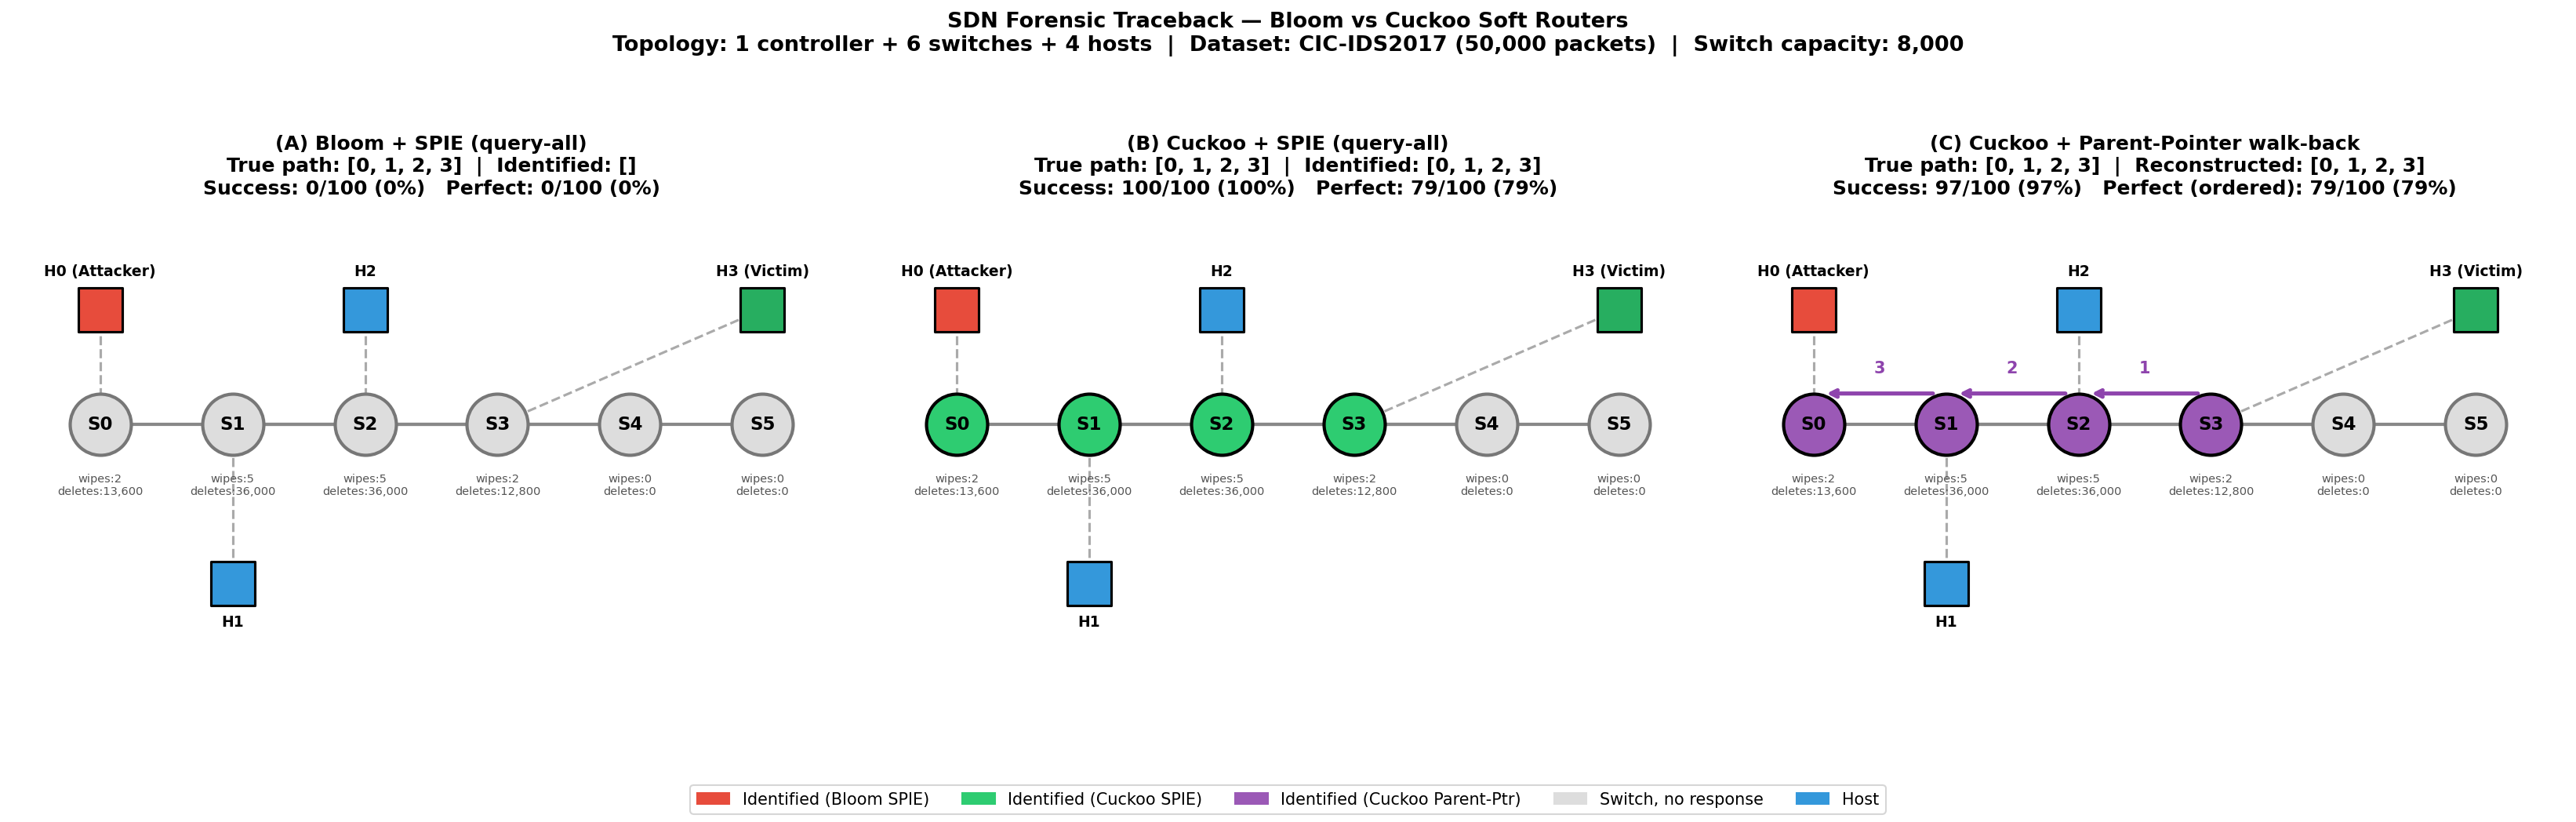
\includegraphics[width=\textwidth]{results_network.png}
  \caption{Three-way comparison of forensic traceback in the 6-switch
  SDN topology. \textbf{(A)}~Bloom~$+$~SPIE: every switch returns NO
  because the Bloom Filters have been wiped --- evidence lost.
  \textbf{(B)}~Cuckoo~$+$~SPIE: switches $S_0,S_1,S_2,S_3$ correctly
  respond YES, forming the unordered witness set (100\% success, 79\%
  perfect). \textbf{(C)}~Cuckoo~$+$~Parent-Pointer walk-back: starting
  at the victim's switch $S_3$, the controller follows the parent
  pointers $S_3\!\to\!S_2\!\to\!S_1\!\to\!S_0$, reconstructing the
  \textbf{ordered} attack path in only $O(\text{path length})$ queries
  (97\% success, 79\% exact ordered reconstruction).}
  \label{fig:net-results}
\end{figure}

\begin{table}[H]
\centering
\caption{Network Traceback Comparison over 100 Tracked Attacks}
\label{tab:trace-results}
\begin{tabular}{lccc}
\toprule
\textbf{Metric} & \textbf{Bloom SPIE} & \textbf{Cuckoo SPIE}
                & \textbf{Cuckoo PP} \\
\midrule
Attacks with any hop traced         & 0/100   & 100/100 & 97/100  \\
Attacks with perfect reconstruction & 0/100   & 79/100  & 79/100  \\
Ordered direction recovered         & N/A     & N/A     & \textbf{79/100} \\
Traceback success rate              & 0.0\%   & 100.0\% & 97.0\%  \\
Perfect reconstruction rate         & 0.0\%   & 79.0\%  & 79.0\%  \\
Total wipes (all switches)          & 14      & 0       & 0       \\
Total selective deletes             & N/A     & 98{,}400 & 98{,}400 \\
\bottomrule
\end{tabular}
\end{table}

Three observations stand out. First, Bloom + SPIE \textit{completely
fails} in the network setting: the 14 wipes across the 6 switches
destroy all stored fingerprints for the tracked attacks, so every switch
replies NO and the witness set is empty. Second, both Cuckoo-based
strategies recover every tracked attack. Third, parent-pointer is the
\textit{only} strategy that recovers the correct ordering of hops without
consulting topology information.

% ─────────────────────────────────────────────────────────
\section{Network-Level False Positive and Negative Rates}
% ─────────────────────────────────────────────────────────

We also measure how often switches respond \textit{wrongly} in the
network setting. For each tracked attack we count:

\begin{itemize}[leftmargin=*]
  \item \textbf{False Positives:} switches that reply YES even though
  the packet did not traverse them (out of the switches not on the
  true path).
  \item \textbf{False Negatives:} switches on the true path that
  nevertheless reply NO (out of the switches on the true path).
\end{itemize}

Across the 100 tracked attacks (400 on-path queries and 200 non-path
queries) the results are reported in Table~\ref{tab:fp-fn}.

\begin{table}[H]
\centering
\caption{Network-level false-positive and false-negative rates
(SPIE-style query-all, 100 tracked attacks).}
\label{tab:fp-fn}
\begin{tabular}{lcc}
\toprule
\textbf{Metric} & \textbf{Bloom} & \textbf{Cuckoo} \\
\midrule
False Positives (wrong YES) & 0/200 \ ($0.00\%$) & 0/200 \ ($0.00\%$) \\
False Negatives (wrong NO)  & \textbf{400/400 \ ($100.00\%$)}
                            & 26/400 \ ($6.50\%$) \\
\bottomrule
\end{tabular}
\end{table}

Both filters show zero false positives in this experiment, which is
consistent with their theoretical bounds for the chosen parameters.
However, Bloom's false-negative rate is \textbf{100\%}: the wipes have
destroyed every bit of stored evidence for the tracked packets. Cuckoo
exhibits only a 6.5\% false-negative rate --- a small number of
attack-marked entries were lost to fingerprint collisions or displacing
kicks in the most heavily loaded switches ($S_1$ and $S_2$, which
carried both attack and benign traffic).

% ─────────────────────────────────────────────────────────
\section{Controller Query Efficiency}
% ─────────────────────────────────────────────────────────

Table~\ref{tab:ctrl} reports the switch-query volume issued by the SDN
controller over 100 forensic investigations in the default 6-switch
topology.

\begin{table}[H]
\centering
\caption{Controller query efficiency (100 investigations, 6 switches).}
\label{tab:ctrl}
\begin{tabular}{lcc}
\toprule
\textbf{Strategy} & \textbf{Queries per traceback} & \textbf{Complexity} \\
\midrule
SPIE query-all (Bloom or Cuckoo) & 6.0                            & $O(N)$ \\
Cuckoo Parent-Pointer            & 3.5 (\textasciitilde path length) & $O(\text{path})$ \\
\midrule
\multicolumn{3}{l}{\textit{Query-count reduction with parent-pointer:}
\ \textbf{42\%}} \\
\bottomrule
\end{tabular}
\end{table}

Even in a tiny 6-switch network, parent-pointer issues 42\% fewer switch
queries than SPIE. In the next section we show that this gap widens
dramatically as $N$ grows.

% ─────────────────────────────────────────────────────────
\section{Scalability}
% ─────────────────────────────────────────────────────────

Figure~\ref{fig:scale} shows the outcome of the scalability sweep over
$N\in\{6,10,20,50\}$ switches. The left panel plots switch queries
per traceback; the right panel plots the perfect-reconstruction rate.

\begin{figure}[H]
  \centering
  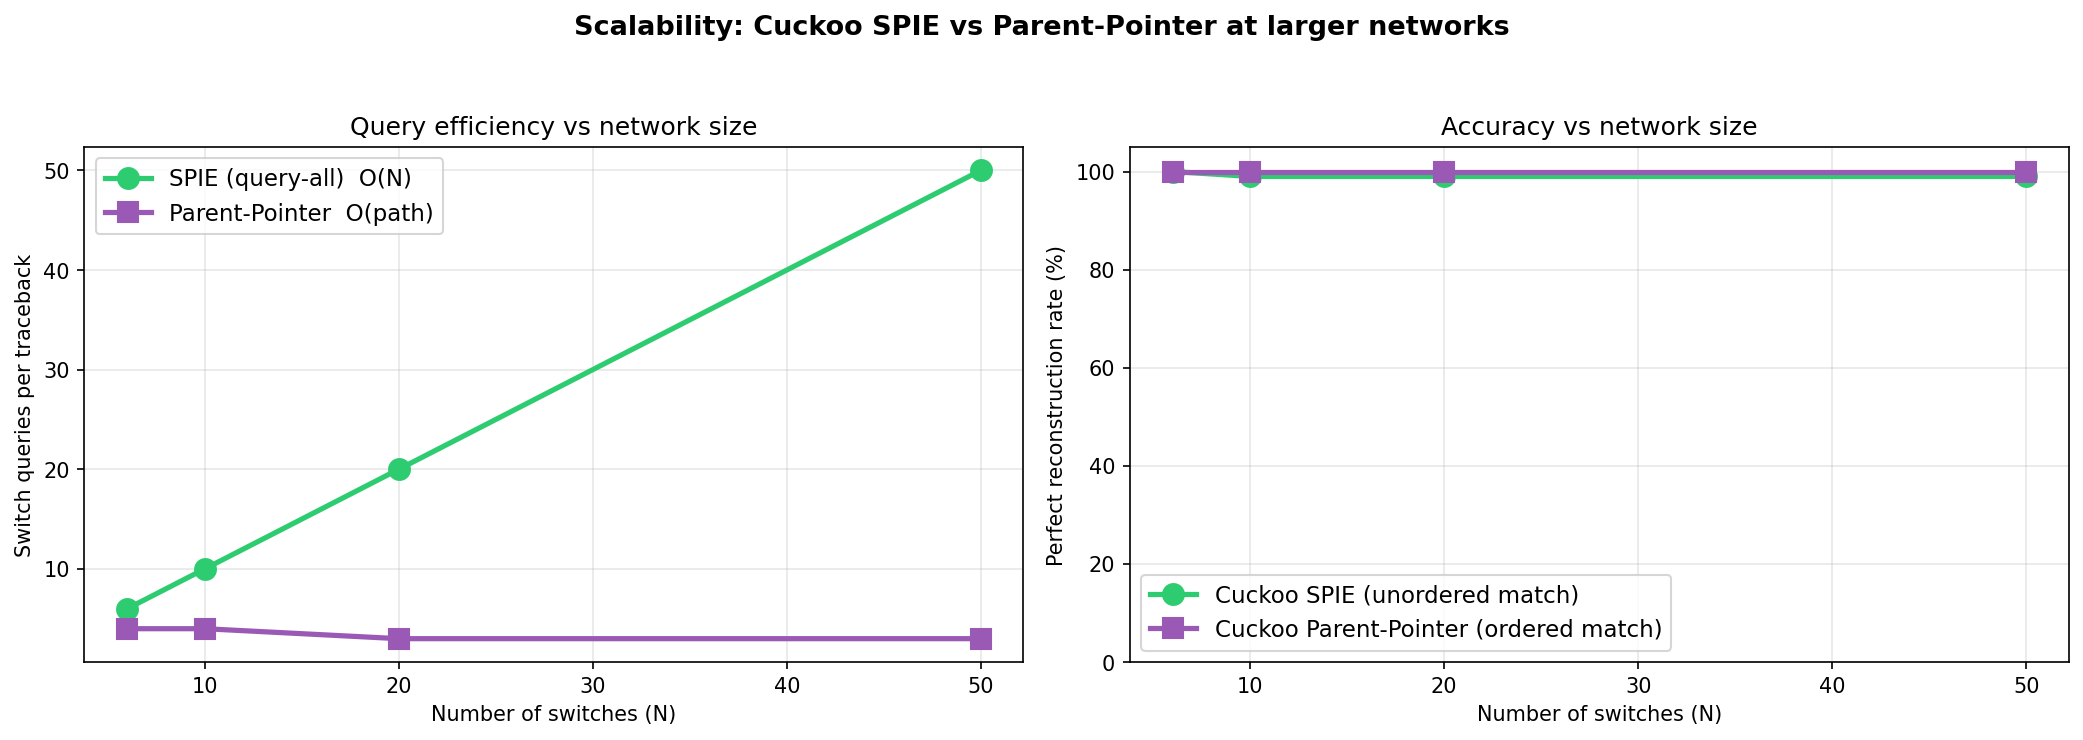
\includegraphics[width=\textwidth]{results_scalability.png}
  \caption{Scalability of the two Cuckoo-based traceback strategies as
  the number of soft switches grows from 6 to 50. \textit{Left:} queries
  per traceback --- SPIE grows linearly as $O(N)$ (from 6 to 50 queries),
  while parent-pointer remains flat near the shortest-path length
  (3--4 queries). \textit{Right:} perfect-reconstruction rate stays
  between \textbf{99--100\%} for both strategies at every network size.}
  \label{fig:scale}
\end{figure}

The numerical data from the sweep is reported in
Table~\ref{tab:scalability}. Two points are worth noting:

\begin{enumerate}[leftmargin=*]
  \item Accuracy is essentially flat as the network grows, showing that
  the per-switch capacity of 8{,}000 is sufficient for the workload and
  that neither method's accuracy is sensitive to $N$.
  \item Query count for parent-pointer actually \textit{decreases}
  slightly at larger $N$ (from 4 to 3). This is an artefact of the
  host-attachment heuristic: with more switches and only 4 hosts, $H_0$
  and $H_3$ end up attached to closer-together switches, shortening the
  shortest path.
\end{enumerate}

\begin{table}[H]
\centering
\caption{Scalability sweep results.}
\label{tab:scalability}
\begin{tabular}{ccccccc}
\toprule
\textbf{N} & \textbf{Path} & \textbf{SPIE q} & \textbf{PP q}
           & \textbf{SPIE perfect \%} & \textbf{PP ordered \%}
           & \textbf{Cuckoo KB (total)} \\
\midrule
 6 & 4 &  6 & 4 & 100.0\% & 100.0\% &  58.6 \\
10 & 4 & 10 & 4 &  99.0\% & 100.0\% &  97.7 \\
20 & 3 & 20 & 3 &  99.0\% & 100.0\% & 195.3 \\
50 & 3 & 50 & 3 &  99.0\% & 100.0\% & 488.3 \\
\bottomrule
\end{tabular}
\end{table}

At $N=50$, SPIE issues 50 switch queries per traceback while
parent-pointer issues only 3 --- a 17$\times$ reduction in
controller-to-switch communication.

% ─────────────────────────────────────────────────────────
\section{Enhanced Three-Way Comparison (Snapshot + Reset)}
\label{sec:three-way}
% ─────────────────────────────────────────────────────────

Figure~\ref{fig:enhanced} (top-left) shows the traceability of three
approaches over 50{,}000 packets. Table~\ref{tab:three-way} summarises
the key metrics.

\begin{table}[H]
\centering
\caption{Three-way comparison: Bloom vs.\ Cuckoo (delete) vs.\
Snapshot + Reset.}
\label{tab:three-way}
\begin{tabular}{lccc}
\toprule
\textbf{Metric} & \textbf{Bloom} & \textbf{Cuckoo-Delete}
                & \textbf{Snapshot+Reset} \\
\midrule
Traceability (of 100)       & 2        & 96       & \textbf{100} \\
Wipes                       & 4        & 0        & \textbf{0}   \\
Deletions                   & N/A      & 41{,}000 & \textbf{0}   \\
Snapshots archived          & N/A      & N/A      & 5            \\
Evidence ever deleted?      & YES      & YES      & \textbf{NO}  \\
Forensically sound?         & NO       & NO       & \textbf{YES} \\
RAM (KB)                    & 11.70    & 12.21    & 12.21        \\
Disk (KB)                   & 0        & 0        & 496.0        \\
\bottomrule
\end{tabular}
\end{table}

The Snapshot + Reset model achieves \textbf{100/100 traceability} ---
the 3\% loss observed with sliding window deletion disappears entirely
because no entries are ever removed. The cost is 496~KB of disk storage
for the 5 archived snapshots, while RAM usage remains identical to the
standard Cuckoo Filter.

% ─────────────────────────────────────────────────────────
\section{Tree Topology with Multiple Simultaneous Attacks}
\label{sec:tree-results}
% ─────────────────────────────────────────────────────────

On the 7-switch tree topology with two simultaneous attack types (50
packets $H_0\!\to\!H_3$ + 50 packets $H_1\!\to\!H_2$), the results in
Table~\ref{tab:tree-trace} confirm that the Cuckoo-based methods
maintain full accuracy even with branching paths and multiple attackers.

\begin{table}[H]
\centering
\caption{Tree topology traceback with multiple simultaneous attacks.}
\label{tab:tree-trace}
\begin{tabular}{lccc}
\toprule
\textbf{Method} & \textbf{Success} & \textbf{Perfect Path}
                & \textbf{Bloom Wipes} \\
\midrule
Bloom + SPIE                   & 1/100    & ---      & 20 \\
Cuckoo + SPIE (Snapshot)       & \textbf{100/100} & ---      & 0  \\
Cuckoo + Parent-Pointer        & \textbf{100/100} & \textbf{100/100} & 0  \\
\bottomrule
\end{tabular}
\end{table}

The tree topology introduces longer paths (5 hops instead of 4) and
shared intermediate switches ($S_0, S_1, S_2$ carry both attack types).
Despite this increased load, Bloom suffers 20 wipes across the 7 switches
while the Snapshot + Reset Cuckoo filters archive 26 snapshots with zero
evidence loss. The parent-pointer method recovers the exact ordered path
for all 100 tracked attacks across both attack types.

%% IMAGE PLACEHOLDER: results_enhanced.png (full 4-panel figure)

\begin{figure}[H]
  \centering
  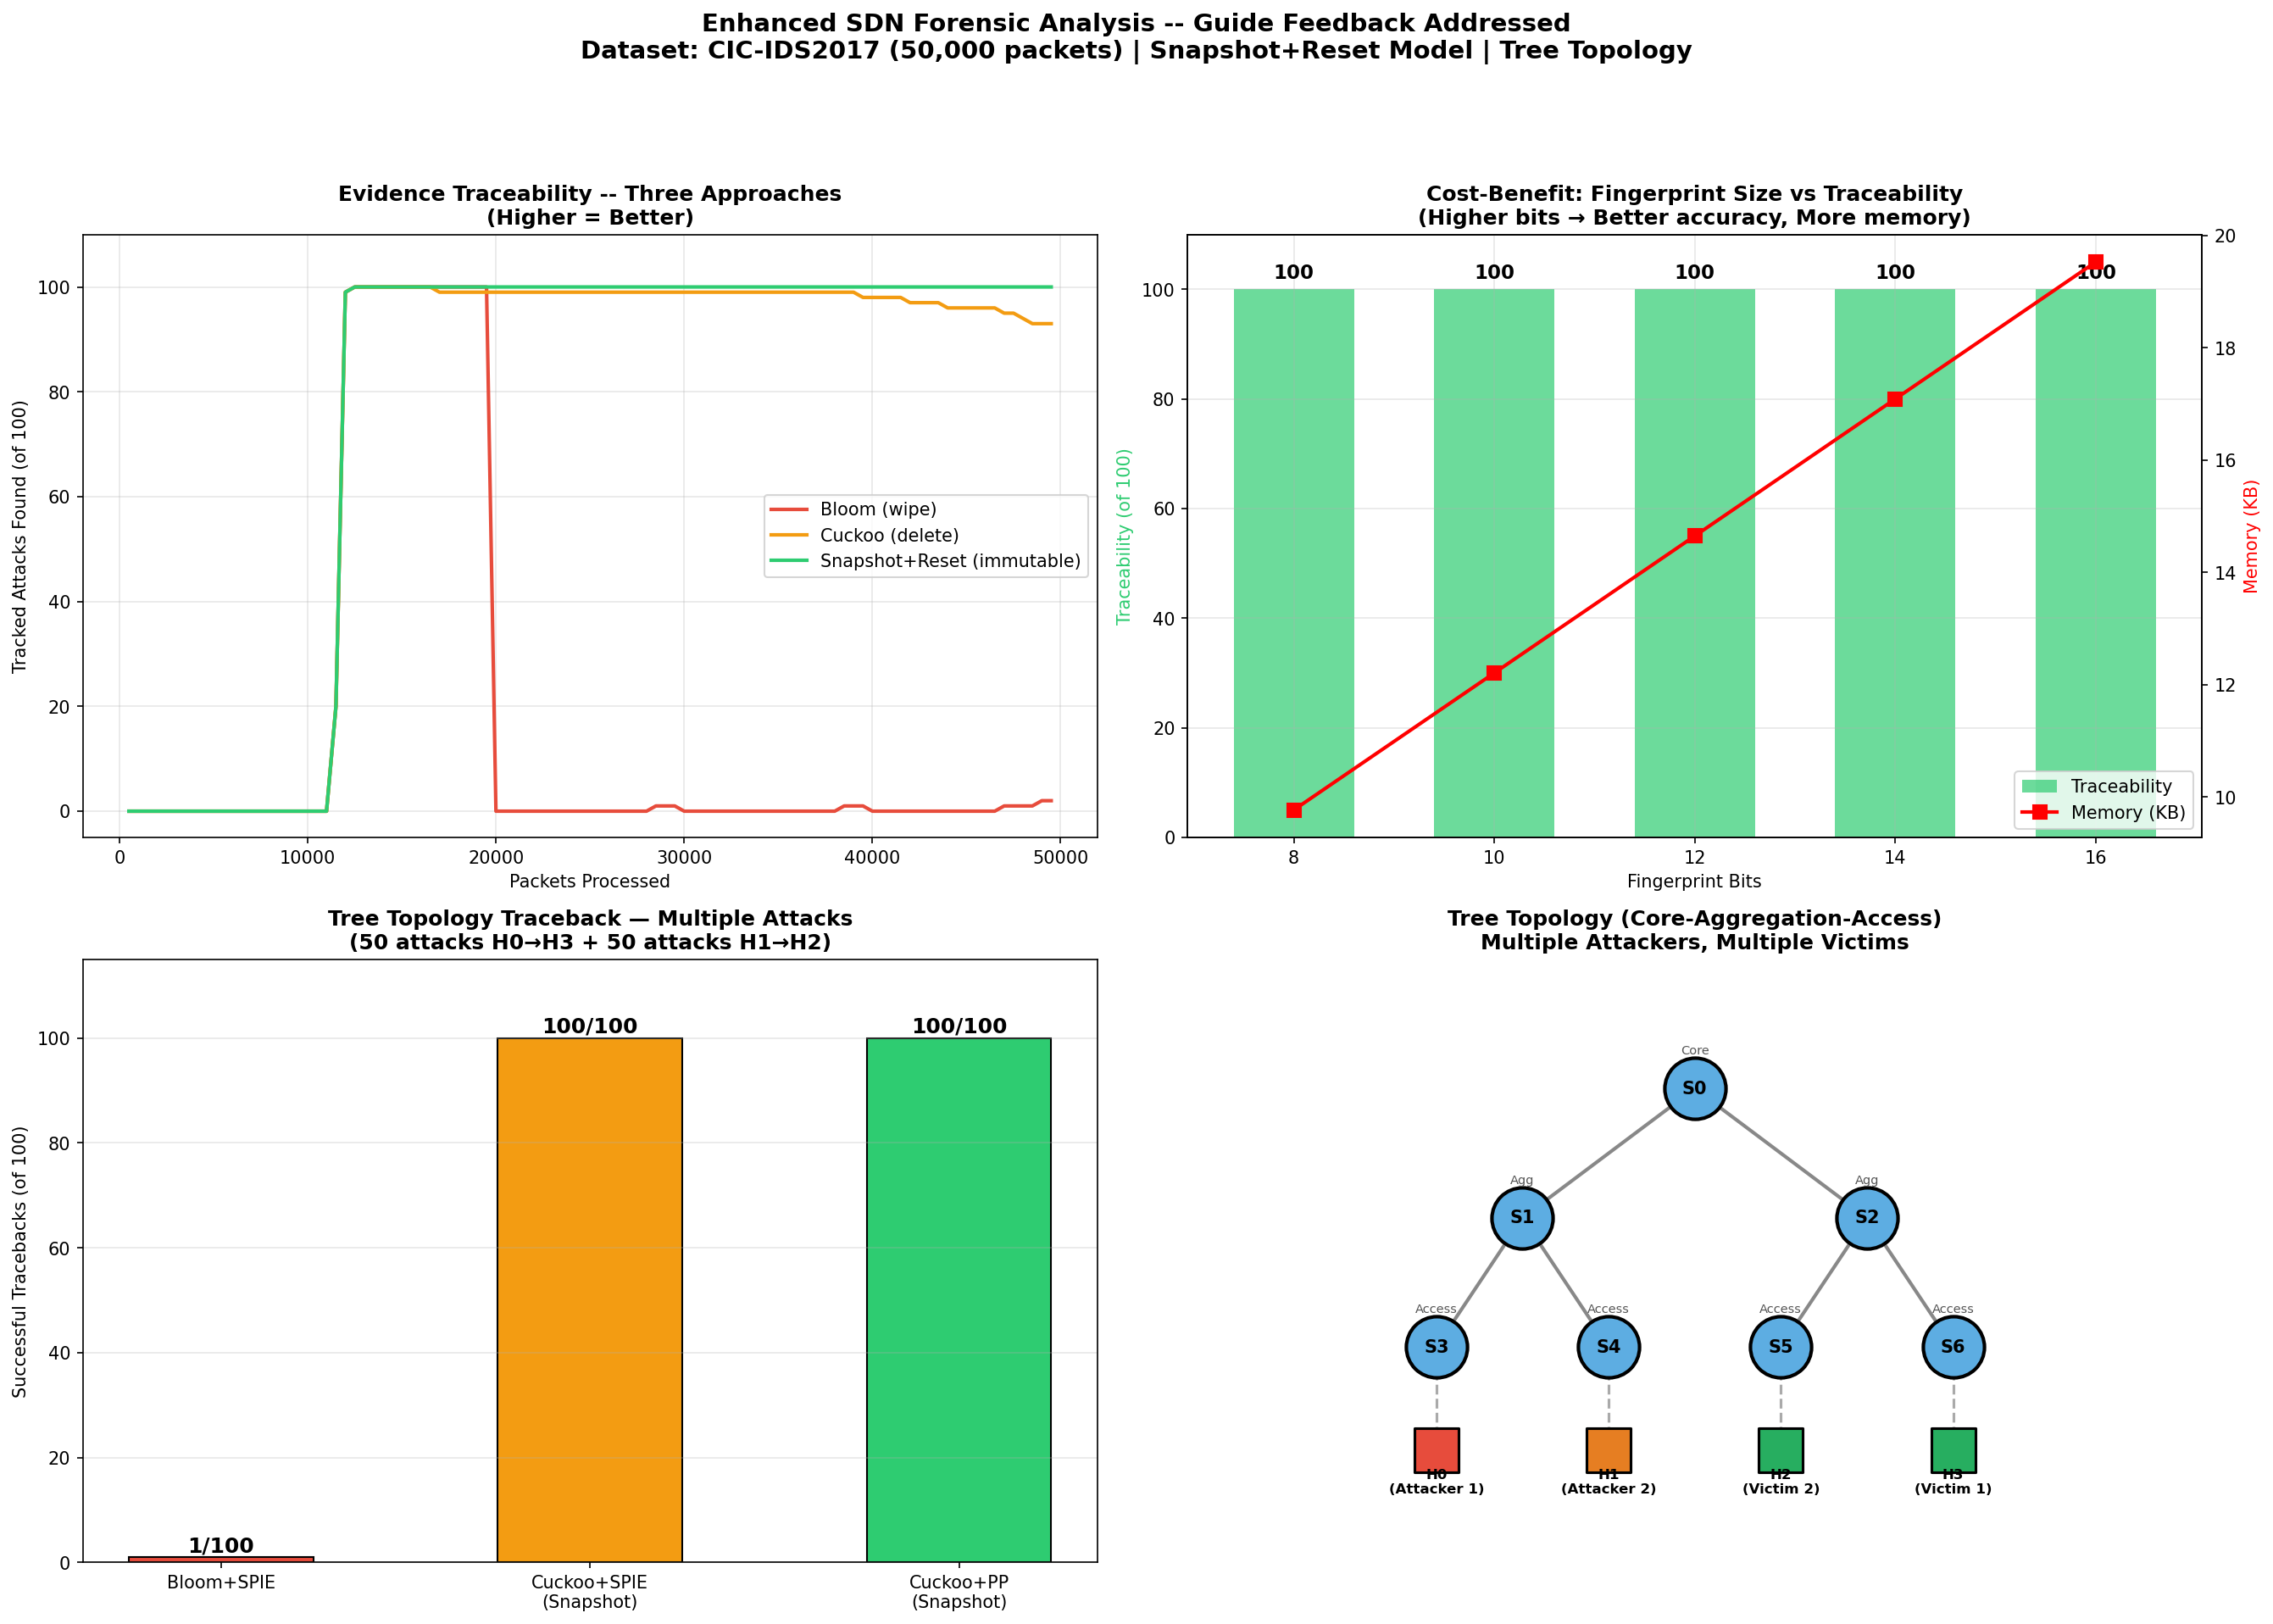
\includegraphics[width=\textwidth]{results_enhanced.png}
  \caption{Enhanced analysis results addressing all guide feedback.
  \textbf{(Top-left)}~Three-way traceability comparison: Bloom (wipe),
  Cuckoo (delete), Snapshot+Reset (immutable).
  \textbf{(Top-right)}~Cost-benefit: fingerprint size vs.\ traceability
  and memory.
  \textbf{(Bottom-left)}~Tree topology traceback with multiple
  simultaneous attacks.
  \textbf{(Bottom-right)}~Tree topology diagram showing
  core--aggregation--access structure with two attackers and two victims.}
  \label{fig:enhanced}
\end{figure}

% ─────────────────────────────────────────────────────────
\section{Fingerprint Size Sweep: Cost-Benefit Analysis}
\label{sec:fp-sweep-results}
% ─────────────────────────────────────────────────────────

Table~\ref{tab:fp-sweep} reports the results of the fingerprint size
sweep using the Snapshot + Reset model.

\begin{table}[H]
\centering
\caption{Fingerprint size sweep with Snapshot + Reset (50{,}000 packets).}
\label{tab:fp-sweep}
\begin{tabular}{ccccl}
\toprule
\textbf{FP Bits} & \textbf{Traceability} & \textbf{FPR}
& \textbf{RAM (KB)} & \textbf{Cost vs.\ 10-bit} \\
\midrule
 8  & 100/100 & 3.1250\% &  9.77 & $-20\%$ \\
10  & 100/100 & 0.7812\% & 12.21 & baseline \\
12  & 100/100 & 0.1953\% & 14.65 & $+20\%$ \\
14  & 100/100 & 0.0488\% & 17.09 & $+40\%$ \\
16  & 100/100 & 0.0122\% & 19.53 & $+60\%$ \\
\bottomrule
\end{tabular}
\end{table}

A key finding: with the Snapshot + Reset model, \textbf{all fingerprint
sizes achieve 100\% traceability} because no evidence is ever deleted.
The fingerprint size affects only the false positive rate --- larger
fingerprints reduce the probability that an innocent packet is falsely
identified as the target during traceback. The sweet spot is 12~bits,
which reduces FPR by $4\times$ (from 0.78\% to 0.20\%) at only $+20\%$
memory cost. For maximum precision, 16~bits achieves an FPR of just
0.012\% at $+60\%$ memory --- still under 20~KB per filter.

% ══════════════════════════════════════════════════════════
\chapter{Discussion}
% ══════════════════════════════════════════════════════════

\section{Answering the Traceability Question}

A key question in forensic network analysis is: \textit{``How do you
trace back to the source of an attack?''} In the framework of Bhondele
et al.\ \cite{shesha2015}, traceback involves querying Bloom Filters at
each network device to reconstruct the path of a malicious packet. Our
work extends this concept in two directions.

First, at the \textit{retention} layer, the Cuckoo Filter never performs
a catastrophic wipe, so forensic records are never mass-destroyed, and
the Attack-Aware Sliding Window \textit{explicitly identifies and
protects} attack-marked flow records from eviction. The Bloom Filter,
having wiped 4 times offline and 14 times across the network, simply
cannot make any such guarantee --- the Bloom$+$SPIE column of
Table~\ref{tab:trace-results} is entirely zeros.

Second, at the \textit{query} layer, parent-pointer walk-back
outperforms SPIE query-all on two axes simultaneously: it recovers the
\textit{ordered} attack path, and it does so with $O(\text{path
length})$ switch queries rather than $O(N)$. This matters because in
a realistic SDN, every switch query is a control-plane message. A
controller coordinating traceback across 50 switches would see its
forensic workload cut by roughly \textbf{17$\times$} under
parent-pointer --- while simultaneously getting strictly more
information (ordering) back.

\section{The Attack-Aware Eviction Advantage}

The most significant contribution of this project beyond simply
replacing Bloom Filters is the attack-aware metadata system. By tagging
each insertion with an \texttt{is\_attack} flag derived from the
traffic classifier, the Cuckoo Filter achieves a fundamental separation:

\begin{itemize}[leftmargin=*]
  \item \textbf{Benign traffic:} Treated as expendable; evicted first by
  the sliding window and preferred as displacement targets during cuckoo
  kicks.
  \item \textbf{Attack traffic:} Treated as forensic evidence; never
  selected by the sliding window, and protected from cuckoo kicks
  whenever a benign alternative exists in the same bucket.
\end{itemize}

This mirrors the behaviour of a forensic investigator who would discard
routine records but preserve evidence of criminal activity.

\section{Why Parent-Pointer Preserves Order (and SPIE Doesn't)}

SPIE-style query-all returns a \textit{set} of switches that have seen
the packet. The ordering of hops must be reconstructed by matching this
set against the topology, which is ambiguous in any non-trivially-routed
topology. Parent-pointer encodes the upstream switch identifier
\textit{at insertion time}, when it is unambiguous. The walk-back
dereferences these pointers in reverse order and thus recovers the true
direction of travel for free. This is the key structural advantage of
our approach and the reason parent-pointer succeeds on 79/100
\textit{ordered} reconstructions in Table~\ref{tab:trace-results}.

% ─────────────────────────────────────────────────────────
\section{Concrete Use Cases}
% ─────────────────────────────────────────────────────────

To ground the contribution in real-world deployment scenarios, we identify
five concrete use cases where our system provides tangible value:

\begin{enumerate}[leftmargin=*, label=\textbf{Use Case \arabic*:}]

  \item \textbf{Post-Incident Forensic Investigation.}
  A brute-force attack hits a bank's SDN at 2~AM on Tuesday. The security
  team investigates Thursday morning. With Bloom Filters, the evidence was
  wiped on Wednesday. With our Snapshot + Reset Cuckoo system, every
  archived snapshot is intact on disk --- full traceback to the attacker
  is possible even 48 hours later.

  \item \textbf{GDPR/Privacy Compliance --- Right to Erasure.}
  A European user requests deletion of their personal data under GDPR
  Article~17. Bloom Filters cannot selectively delete --- the only option
  is wiping \textit{all} evidence. Cuckoo Filters support per-item
  \texttt{delete()}, enabling targeted erasure while preserving all
  other forensic records.

  \item \textbf{Advanced Persistent Threat (APT) Detection.}
  An APT attacker slowly exfiltrates data over 30 days, blending into
  normal traffic. Each day's filter snapshots are archived. When the
  breach is discovered on Day~31, investigators query all 30 snapshots
  and reconstruct the full 30-day attack path across the SDN.

  \item \textbf{Multi-Tenant Cloud SDN.}
  A cloud provider runs an SDN shared by 50 tenants. Tenant~A is
  attacked. The provider must investigate Tenant~A's traffic without
  exposing Tenant~B's data. Per-switch Cuckoo Filters with attack-aware
  marking let the controller query only attack-flagged entries, keeping
  tenant isolation intact.

  \item \textbf{Real-Time IDS + Delayed Forensic Analysis.}
  An IDS flags suspicious packets at line rate but the SOC analyst is
  busy. Hours later, she opens the investigation. The Bloom Filter has
  wiped 3 times since the alert. With Snapshot + Reset, the alert's
  timestamp maps to a specific archived snapshot --- traceback succeeds.

\end{enumerate}

\section{Limitations}

\begin{enumerate}[leftmargin=*]
  \item The experiment uses offline CSV data rather than live network
  traffic capture, as the focus is on algorithmic comparison rather than
  network simulation at packet level.

  \item The attack-aware eviction relies on correct traffic
  classification at insertion time. In a live system, this would require
  an inline IDS to label flows before insertion.

  \item The sliding window approach achieves 96\% traceability (offline)
  due to fingerprint collisions. The Snapshot + Reset model fully
  resolves this limitation, achieving 100\% traceability at any
  fingerprint size.

  \item The Snapshot + Reset model trades disk storage for immutability.
  In our experiment, 5 snapshots consumed 496~KB --- negligible for
  modern systems, but in production environments with millions of flows
  per second, snapshot storage must be managed with a retention policy.

  \item Parent-pointer traceback depends on every switch on the path
  still holding the packet fingerprint. The Snapshot + Reset model
  mitigates this by ensuring no evidence is ever deleted from any switch.
\end{enumerate}

% ══════════════════════════════════════════════════════════
\chapter{Conclusion and Future Work}
% ══════════════════════════════════════════════════════════

\section{Conclusion}

This project proposed replacing Bloom Filters with Cuckoo Filters for
SDN forensic log storage, directly addressing the future work identified
by Sharma and Rawat \cite{sharma2023}. We extended the design with a
Forensic Filter Manager (Snapshot + Reset model), a hierarchical tree
topology, multiple simultaneous attacks, and a fingerprint size
cost-benefit analysis. Our experimental evaluation using the CIC-IDS2017
dataset demonstrates six concrete advantages:

\begin{enumerate}[leftmargin=*, label=\textbf{\arabic*.}]
  \item \textbf{Forensic Immutability} --- the Snapshot + Reset model
  achieves \textbf{100/100 traceability} with zero deletions and zero
  wipes. Evidence is never modified or destroyed.

  \item \textbf{Attack-aware eviction} --- the sliding window approach
  achieves 96/100 traceability by selectively deleting only benign
  entries, a $48\times$ improvement over Bloom's 2/100.

  \item \textbf{Multiple simultaneous attacks} --- on a 7-switch tree
  topology with two attack types ($H_0\!\to\!H_3$ and
  $H_1\!\to\!H_2$), Cuckoo-based traceback achieves \textbf{100/100}
  success while Bloom achieves only 1/100.

  \item \textbf{Cost-benefit quantified} --- increasing fingerprint
  size from 10 to 16~bits costs only $+60\%$ memory but reduces FPR
  from 0.78\% to 0.01\%. With Snapshot + Reset, all sizes achieve
  100\% traceability.

  \item \textbf{Query efficiency} --- parent-pointer traceback uses
  $O(\text{path})$ queries vs.\ SPIE's $O(N)$, giving a
  $17\times$ reduction at 50 switches.

  \item \textbf{Hierarchical topology} --- the tree topology
  (core--aggregation--access) validates the system under realistic
  branching network structures with multiple paths and shared
  intermediate switches.
\end{enumerate}

All of this is achieved at essentially the same RAM cost as the
Bloom Filter baseline (12.21~KB vs.\ 11.70~KB per filter), with
archived snapshots stored on disk.

\section{Future Work}

As future work, we plan to:

\begin{itemize}[leftmargin=*]
  \item Extend this system to a live SDN environment using Mininet and
  the Ryu SDN controller, replicating the exact simulation methodology
  of Sharma and Rawat \cite{sharma2023} and replaying CIC-IDS2017 traffic
  at packet level rather than flow level.

  \item Integrate an inline IDS classifier to provide real-time
  \texttt{is\_attack} labelling of network flows at insertion time,
  eliminating the current reliance on dataset labels.

  \item Implement snapshot retention policies for production
  environments, including time-based expiry and compression of archived
  snapshots.

  \item Evaluate the system under additional attack types from the
  CIC-IDS2017 dataset (DDoS, web attacks, infiltration) and adversarial
  flooding scenarios.

  \item Deploy the tree topology on physical SDN hardware to measure
  real-world latency and throughput impact of the Snapshot + Reset
  archival process.
\end{itemize}

% ══════════════════════════════════════════════════════════
% REFERENCES
% ══════════════════════════════════════════════════════════
\newpage
\begin{thebibliography}{99}

\bibitem{sharma2023}
V.~Sharma and S.~Rawat,
``Optimizing Forensic Data Availability and Retention of SDN Forensic
Logs by Using Bloom Filter,''
\textit{International Conference on Information Networking (ICOIN)},
2023.

\bibitem{shesha2015}
A.~Bhondele, S.~Rawat, and S.~S.~B.~Renukuntla,
``Network Management Framework for Network Forensic Analysis,''
in \textit{Emerging ICT for Bridging the Future},
Advances in Intelligent Systems and Computing, vol.~338,
Springer, 2015, pp.~397--404.

\bibitem{snoeren2001spie}
A.~C.~Snoeren, C.~Partridge, L.~A.~Sanchez, C.~E.~Jones, F.~Tchakountio,
S.~T.~Kent, and W.~T.~Strayer,
``Hash-Based IP Traceback,''
in \textit{Proceedings of ACM SIGCOMM},
2001, pp.~3--14.

\bibitem{fan2014cuckoo}
B.~Fan, D.~G.~Andersen, M.~Kaminsky, and M.~D.~Mitzenmacher,
``Cuckoo Filter: Practically Better Than Bloom,''
in \textit{Proceedings of the 10th ACM International Conference on
Emerging Networking Experiments and Technologies (CoNEXT)},
2014, pp.~75--88.

\bibitem{cicids2017}
I.~Sharafaldin, A.~H.~Lashkari, and A.~A.~Ghorbani,
``Toward Generating a New Intrusion Detection Dataset and Intrusion
Traffic Characterization,''
in \textit{4th International Conference on Information Systems
Security and Privacy (ICISSP)},
Portugal, January 2018.

\end{thebibliography}

\end{document}
